    %Version 3.1 December 2024
% See section 11 of the User Manual for version history
%
%%%%%%%%%%%%%%%%%%%%%%%%%%%%%%%%%%%%%%%%%%%%%%%%%%%%%%%%%%%%%%%%%%%%%%
%%                                                                 %%
%% Please do not use \input{...} to include other tex files.       %%
%% Submit your LaTeX manuscript as one .tex document.              %%
%%                                                                 %%
%% All additional figures and files should be attached             %%
%% separately and not embedded in the \TeX\ document itself.       %%
%%                                                                 %%
%%%%%%%%%%%%%%%%%%%%%%%%%%%%%%%%%%%%%%%%%%%%%%%%%%%%%%%%%%%%%%%%%%%%%

%%\documentclass[referee,sn-basic]{sn-jnl}% referee option is meant for double line spacing

%%=======================================================%%
%% to print line numbers in the margin use lineno option %%
%%=======================================================%%

%%\documentclass[lineno,pdflatex,sn-basic]{sn-jnl}% Basic Springer Nature Reference Style/Chemistry Reference Style

%%=========================================================================================%%
%% the documentclass is set to pdflatex as default. You can delete it if not appropriate.  %%
%%=========================================================================================%%

%%\documentclass[sn-basic]{sn-jnl}% Basic Springer Nature Reference Style/Chemistry Reference Style

%%Note: the following reference styles support Namedate and Numbered referencing. By default the style follows the most common style. To switch between the options you can add or remove “Numbered” in the optional parenthesis. 
%%The option is available for: sn-basic.bst, sn-chicago.bst%  
 
%%\documentclass[pdflatex,sn-nature]{sn-jnl}% Style for submissions to Nature Portfolio journals
%%\documentclass[pdflatex,sn-basic]{sn-jnl}% Basic Springer Nature Reference Style/Chemistry Reference Style
\documentclass[pdflatex,sn-mathphys-num]{sn-jnl}% Math and Physical Sciences Numbered Reference Style
%%\documentclass[pdflatex,sn-mathphys-ay]{sn-jnl}% Math and Physical Sciences Author Year Reference Style
%%\documentclass[pdflatex,sn-aps]{sn-jnl}% American Physical Society (APS) Reference Style
%%\documentclass[pdflatex,sn-vancouver-num]{sn-jnl}% Vancouver Numbered Reference Style
%%\documentclass[pdflatex,sn-vancouver-ay]{sn-jnl}% Vancouver Author Year Reference Style
%%\documentclass[pdflatex,sn-apa]{sn-jnl}% APA Reference Style
%%\documentclass[pdflatex,sn-chicago]{sn-jnl}% Chicago-based Humanities Reference Style

%%%% Standard Packages
%%<additional latex packages if required can be included here>

\usepackage{graphicx}%
\graphicspath{{figures/}}
\usepackage{multirow}%
\usepackage{amsmath,amssymb,amsfonts}%
\usepackage{amsthm}%
\usepackage{mathrsfs}%
\usepackage[title]{appendix}%
\usepackage{xcolor}%
\usepackage{textcomp}%
\usepackage{manyfoot}%
\usepackage{booktabs}%
\usepackage{algorithm}%
\usepackage{algorithmicx}%
\usepackage{algpseudocode}%
\usepackage{listings}%
\usepackage{longtable}%
\usepackage{array}%
\usepackage{ragged2e}%

\newcolumntype{L}[1]{>{\RaggedRight\arraybackslash}p{#1}}
\usepackage{tikz}%
\usetikzlibrary{positioning,fit,calc,arrows.meta}%
\usepackage{placeins}%
%%%%

%%%%%=============================================================================%%%%
%%%%  Remarks: This template is provided to aid authors with the preparation
%%%%  of original research articles intended for submission to journals published 
%%%%  by Springer Nature. The guidance has been prepared in partnership with 
%%%%  production teams to conform to Springer Nature technical requirements. 
%%%%  Editorial and presentation requirements differ among journal portfolios and 
%%%%  research disciplines. You may find sections in this template are irrelevant 
%%%%  to your work and are empowered to omit any such section if allowed by the 
%%%%  journal you intend to submit to. The submission guidelines and policies 
%%%%  of the journal take precedence. A detailed User Manual is available in the 
%%%%  template package for technical guidance.
%%%%%=============================================================================%%%%

%% as per the requirement new theorem styles can be included as shown below
\theoremstyle{thmstyleone}%
\newtheorem{theorem}{Theorem}%  meant for continuous numbers
%%\newtheorem{theorem}{Theorem}[section]% meant for sectionwise numbers
%% optional argument [theorem] produces theorem numbering sequence instead of independent numbers for Proposition
\newtheorem{proposition}[theorem]{Proposition}% 
%%\newtheorem{proposition}{Proposition}% to get separate numbers for theorem and proposition etc.

\theoremstyle{thmstyletwo}%
\newtheorem{example}{Example}%
\newtheorem{remark}{Remark}%

\theoremstyle{thmstylethree}%
\newtheorem{definition}{Definition}%

\raggedbottom
%%\unnumbered% uncomment this for unnumbered level heads

    \begin{document}

\title[Article Title]{Sistemas inteligentes de videovigilancia y técnicas de Inteligencia
Artificial para la detección y seguimiento de actividades delictivas una Revisión Sistemática de la Literatura.}

%%=============================================================%%
%% GivenName -> \fnm{Nombre}
%% FamilyName -> \sur{Apellido}
%%=============================================================%%

\author*[1]{\fnm{Mixel} \sur{Meza}}\email{prantxes.meza@upeu.edu.pe}

\author[1]{\fnm{Juan} \sur{Espiritu}}\email{juan.espiritu@upeu.edu.pe}

\author[1]{\fnm{Miguel} \sur{Godoy}}\email{miguel.godoy@upeu.edu.pe}

\author[1]{\fnm{Juan Jesús} \sur{Soria Quijaite}}\email{jesussoria@upeu.edu.pe}

\affil*[1]{
\orgdiv{Facultad de Ingeniería y Arquitectura},
\orgname{Universidad Peruana Unión},
\orgaddress{
\city{Lima},
\state{Lima},
\country{Perú}
}}
    
%%==================================%%
%% Sample for unstructured abstract %%
%%==================================%%

\abstract{The abstract serves both as a general introduction to the topic and as a brief, non-technical summary of the main results and their implications. Authors are advised to check the author instructions for the journal they are submitting to for word limits and if structural elements like subheadings, citations, or equations are permitted.}

%%================================%%
%% Sample for structured abstract %%
%%================================%%

% \abstract{\textbf{Purpose:} The abstract serves both as a general introduction to the topic and as a brief, non-technical summary of the main results and their implications. The abstract must not include subheadings (unless expressly permitted in the journal's Instructions to Authors), equations or citations. As a guide the abstract should not exceed 200 words. Most journals do not set a hard limit however authors are advised to check the author instructions for the journal they are submitting to.
% 
% \textbf{Methods:} The abstract serves both as a general introduction to the topic and as a brief, non-technical summary of the main results and their implications. The abstract must not include subheadings (unless expressly permitted in the journal's Instructions to Authors), equations or citations. As a guide the abstract should not exceed 200 words. Most journals do not set a hard limit however authors are advised to check the author instructions for the journal they are submitting to.
% 
% \textbf{Results:} The abstract serves both as a general introduction to the topic and as a brief, non-technical summary of the main results and their implications. The abstract must not include subheadings (unless expressly permitted in the journal's Instructions to Authors), equations or citations. As a guide the abstract should not exceed 200 words. Most journals do not set a hard limit however authors are advised to check the author instructions for the journal they are submitting to.
% 
% \textbf{Conclusion:} The abstract serves both as a general introduction to the topic and as a brief, non-technical summary of the main results and their implications. The abstract must not include subheadings (unless expressly permitted in the journal's Instructions to Authors), equations or citations. As a guide the abstract should not exceed 200 words. Most journals do not set a hard limit however authors are advised to check the author instructions for the journal they are submitting to.}

\keywords{keyword1, Keyword2, Keyword3, Keyword4}

%%\pacs[JEL Classification]{D8, H51}

%%\pacs[MSC Classification]{35A01, 65L10, 65L12, 65L20, 65L70}

\maketitle

\section{Introducción}\label{sec1}

América Latina sostiene niveles de violencia urbana que ninguna otra región iguala. El \emph{Global Study on Homicide} de la Oficina de las Naciones Unidas contra la Droga y el Delito sitúa en las Américas el 34\,\% de los homicidios registrados en el mundo durante 2021, y ocho de los diez países con las tasas más altas del planeta se ubican en América Latina y el Caribe \cite{unodc2023}. Frente a ese panorama, la respuesta institucional dominante ha sido multiplicar los circuitos cerrados de televisión en el espacio público. La política descansa en un supuesto sencillo: observar de forma permanente disuade la comisión de delitos y facilita su esclarecimiento. El supuesto se cumple a medias. Quien vigila decenas de monitores durante turnos prolongados pierde capacidad de atención en cuestión de minutos, de manera que una proporción considerable de los incidentes se advierte recién cuando alguien revisa la grabación, con el hecho ya consumado \cite{bhatti2021}. La cámara termina operando como archivo forense antes que como mecanismo de prevención.

El aprendizaje profundo aplicado a la visión por computador alteró ese escenario, pues permite que el análisis del flujo de video se ejecute de forma automática y continua. Los detectores convolucionales de una sola etapa, y en particular los de la familia YOLO, localizan armas de fuego y armas blancas sobre imágenes de cámaras de vigilancia con precisiones competitivas \cite{ahmed2022}. Detectar el objeto, sin embargo, no basta cuando lo que interesa es la acción, porque reconocer una agresión exige modelar cómo cambia la escena en el tiempo. Las redes recurrentes dotadas de mecanismos de atención abordaron ese problema al ponderar los fotogramas relevantes de cada secuencia \cite{ullah2021}. Las convoluciones tridimensionales lo hicieron por otra vía, extendiendo el filtro al eje temporal \cite{magdy2023}. Ambas familias superan a los descriptores manuales que las precedieron, aunque su desempeño varía de forma notoria según el conjunto de prueba con el que se evalúen \cite{sernani2021}. Trabajos más recientes incorporaron transformadores de visión junto con aprendizaje estructurado para aliviar la dependencia de anotaciones cuadro a cuadro, impracticables a escala urbana \cite{rendon2023}, y combinaciones de autoatención con memorias convolucionales bidireccionales persiguieron el mismo fin \cite{rendon2021}. Una línea menos poblada trasladó el cómputo hacia el borde de la red. Primero, para detectar armas en cámaras de interior sin enviar el video a un servidor central \cite{berardini2024}. Después, incorporando superresolución para compensar la baja calidad de las capturas \cite{berardini2025}. También con arquitecturas que anteponen el cumplimiento de la normativa de privacidad al rendimiento bruto \cite{barthelemy2024}.
Además de la detección automática de conductas delictivas, los sistemas inteligentes de videovigilancia pueden incorporar técnicas orientadas a la identificación y al seguimiento de las personas involucradas. El seguimiento dentro de una misma cámara permite mantener la trayectoria de un individuo u objeto a lo largo del tiempo, mientras que la re-identificación de personas y el seguimiento multi-cámara permiten asociar apariciones del mismo sujeto entre diferentes cámaras. Estas capacidades resultan especialmente relevantes en entornos urbanos, donde una persona puede abandonar el campo visual de una cámara y aparecer posteriormente en otra.

La abundancia de propuestas no se traduce, sin embargo, en evidencia lista para llevarse a una implementación real. Tres limitaciones lo impiden. La primera es la concentración del esfuerzo experimental en un número reducido de conjuntos de datos de referencia: en el corpus examinado en este trabajo, UCF-Crime sostiene trece de los treinta y cinco estudios incluidos, lo que introduce el riesgo de que las mejoras informadas reflejen un ajuste al banco de pruebas antes que capacidad de generalización. Quienes construyeron conjuntos alternativos advirtieron ese riesgo de forma explícita, sea al grabar agresiones en el transporte público real \cite{ciampi2022}, sea al reunir material de cámaras de vigilancia con presencia de armas \cite{hnoohom2022}. A ello se suma la heterogeneidad de las métricas: exactitud, mAP, AUC y F1 se reportan de manera intercambiable y sobre particiones distintas, de modo que la comparación directa entre publicaciones rara vez resulta legítima. La tercera limitación pesa más que las anteriores para la seguridad ciudadana. Casi ningún estudio describe la arquitectura de despliegue, entendida como la cadena de captura, transmisión, procesamiento y notificación: solo siete de los treinta y cinco estudios que superaron la valoración de calidad aportan evidencia sobre la plataforma en la que el modelo llegaría a operar. Las revisiones publicadas hasta la fecha privilegiaron la taxonomía de técnicas y dedicaron atención marginal a estas condiciones de operación.

El presente artículo aborda esa brecha mediante una revisión sistemática de la literatura, conducida según el protocolo de Kitchenham y Charters para ingeniería de software \cite{kitchenham2007} y reportada conforme a la declaración PRISMA 2020 \cite{page2021}. La pregunta que orienta el estudio es doble: qué modelos y algoritmos de inteligencia artificial y visión por computador se emplean para la detección, identificación y seguimiento de actividades delictivas en sistemas de videovigilancia urbana, y qué beneficios, limitaciones y evidencias de desempeño reportan frente a enfoques tradicionales y modelos de referencia previos. La búsqueda se ejecutó en Web of Science, Scopus y ScienceDirect sobre publicaciones del periodo comprendido entre 2021 y 2026, y recuperó 477 registros; 373 superaron el cribado por título y resumen. Esos estudios fueron valorados con una rúbrica de cinco preguntas de calidad en la que la ausencia de evidencia se puntúa como incumplimiento y no como cumplimiento parcial, criterio deliberadamente exigente que dejó 45 trabajos, de los cuales 35 corresponden al contexto de videovigilancia urbana y constituyen el corpus final. El aporte del trabajo es doble. Por un lado, sistematiza las tareas abordadas, los conjuntos de datos empleados, las arquitecturas implementadas y los resultados informados en esos treinta y cinco estudios. Por otro, documenta de forma explícita qué proporción del corpus sostiene cada afirmación, lo que permite separar los hallazgos consolidados de aquellos que descansan en evidencia aislada. Esa distinción suele quedar fuera de las revisiones previas.

% NOTA: cuando crees las secciones 2 a 5 con sus \label, reemplaza los números
% literales de abajo por \ref{...} para que se numeren solas.
El resto del documento se organiza como sigue. La sección 2 describe el protocolo de revisión, las ecuaciones de búsqueda aplicadas en cada base de datos y los criterios de valoración de la calidad. La sección 3 presenta los resultados agrupados según las cinco preguntas de calidad. La sección 4 discute las implicaciones para el diseño de sistemas de videovigilancia asistida por inteligencia artificial, junto con las limitaciones del propio estudio. La sección 5 recoge las conclusiones.

\section{Metodología}\label{sec2}

\subsection{Diseño de la revisión sistemática}\label{subsec:diseno}

Este estudio se desarrolló como una revisión sistemática de la literatura (RSL). La revisión se planificó y condujo siguiendo las directrices de Kitchenham y Charters para revisiones sistemáticas en ingeniería de software, que organizan el proceso en las etapas de planificación, conducción y reporte \cite{kitchenham2007}. La declaración PRISMA 2020 se utilizó para documentar el flujo de identificación y selección de los estudios, ya que sus autores la conciben como una guía de reporte y no como un procedimiento para conducir revisiones \cite{page2021}. Esta combinación es coherente con las pautas SEGRESS, que adaptan PRISMA 2020 al reporte de estudios secundarios en ingeniería de software \cite{kitchenham2023}. El protocolo, la importación de los registros, la selección de estudios, la evaluación de calidad y la extracción de datos se gestionaron en Parsifal, una plataforma web de apoyo a revisiones sistemáticas.

\subsection{Objetivo y preguntas de investigación}\label{subsec:preguntas}

El objetivo de la revisión fue sintetizar y analizar críticamente la evidencia publicada entre 2021 y 2026 sobre modelos y técnicas de Inteligencia Artificial aplicados a la detección de actividades delictivas y al seguimiento de personas u objetos de interés en sistemas de videovigilancia, considerando las arquitecturas empleadas, los conjuntos de datos, las métricas de desempeño y la evidencia de implementación y despliegue. La revisión se orientó mediante la siguiente pregunta principal: ¿Qué modelos y técnicas de Inteligencia Artificial se han aplicado, entre 2021 y 2026, para la detección y seguimiento de actividades delictivas en sistemas de videovigilancia urbana, incluyendo técnicas de identificación, re-identificación y seguimiento de personas involucradas, y qué resultados de desempeño y evidencias de implementación y despliegue reportan? A partir de ella se formularon cinco preguntas específicas (Tabla~\ref{tab:rq}), que desagregan la pregunta principal en los modelos empleados, los eventos de seguridad y las capacidades de seguimiento abordadas, los conjuntos de datos y escenarios de evaluación, las métricas de desempeño y la evidencia de implementación y despliegue.

\begin{table}[h]
\hyphenpenalty=10000\exhyphenpenalty=10000
\caption{Preguntas de investigación de la revisión sistemática}\label{tab:rq}
\begin{tabular}{@{}L{1.0cm}L{11.5cm}@{}}
\toprule
Código & Pregunta \\
\midrule
RQ1 & ¿Qué modelos, algoritmos y arquitecturas de Inteligencia Artificial se utilizan para la detección de actividades delictivas y para la identificación, re-identificación y seguimiento de personas involucradas en sistemas de videovigilancia? \\
\addlinespace
RQ2 & ¿Qué tipos de actividades delictivas y eventos de seguridad son detectados por los sistemas inteligentes de videovigilancia, y qué capacidades de identificación, re-identificación y seguimiento de las personas involucradas son abordadas? \\
\addlinespace
RQ3 & ¿Qué conjuntos de datos y escenarios de videovigilancia se utilizan para entrenar y evaluar los modelos de detección de actividades delictivas y de identificación, re-identificación y seguimiento de personas? \\
\addlinespace
RQ4 & ¿Qué métricas y niveles de desempeño reportan los modelos de Inteligencia Artificial aplicados a la detección de actividades delictivas y a la identificación, re-identificación y seguimiento de personas? \\
\addlinespace
RQ5 & ¿Qué evidencia de implementación, procesamiento en tiempo real, arquitectura de despliegue y limitaciones reportan los sistemas inteligentes de videovigilancia para la detección y seguimiento de actividades delictivas? \\
\bottomrule
\end{tabular}
\end{table}

\subsection{Estrategia PICOC}\label{subsec:picoc}

La pregunta se delimitó con el marco PICOC (población, intervención, comparación, resultados y contexto), descrito por Petticrew y Roberts para estructurar preguntas de revisión \cite{petticrew2006} y recogido por Kitchenham y Charters para la ingeniería de software \cite{kitchenham2007}. La Tabla~\ref{tab:picoc} presenta los cinco componentes registrados en el protocolo. El periodo 2021--2026 no se trató como un componente adicional del marco, sino como una delimitación temporal que se aplicó mediante los filtros de búsqueda.

\begin{table}[h]
\hyphenpenalty=10000\exhyphenpenalty=10000
\caption{Componentes PICOC definidos en el protocolo}\label{tab:picoc}
\begin{tabular}{@{}L{2.4cm}L{10.1cm}@{}}
\toprule
Componente & Definición registrada en el protocolo \\
\midrule
Población (P) & Actividades delictivas y eventos de seguridad observados mediante sistemas de videovigilancia, incluyendo personas u objetos de interés relacionados con dichos eventos. \\
\addlinespace
Intervención (I) & Inteligencia Artificial, aprendizaje automático/profundo y visión por computador aplicados a detección de actividades delictivas y seguimiento de personas u objetos de interés en eventos de seguridad. \\
\addlinespace
Comparación (C) & Monitoreo humano tradicional de videovigilancia, sistemas CCTV sin Inteligencia Artificial, métodos convencionales basados en características manuales, modelos \textit{baseline}. \\
\addlinespace
Resultados (O) & Accuracy, Precision, Recall, F1-Score, mAP, AUC, métricas de seguimiento como MOTA, MOTP, IDF1 y HOTA, así como FPS y latencia. \\
\addlinespace
Contexto (C) & Sistemas de videovigilancia orientados a seguridad en espacios públicos y entornos urbanos. \\
\bottomrule
\end{tabular}
\end{table}

\subsection{Estrategia de búsqueda}\label{subsec:busqueda}

Los términos de búsqueda se derivaron de los componentes PICOC y se registraron en el protocolo como términos en inglés agrupados por concepto (Tabla~\ref{tab:keywords}). Las filas de esa tabla indican el componente PICOC al que se vinculó cada concepto. A partir de los conceptos registrados se construyó la cadena base de búsqueda. La cadena base se organizó en tres bloques: videovigilancia, Inteligencia Artificial y eventos de seguridad. Los términos de cada bloque se combinaron con OR y los bloques se relacionaron mediante AND, procedimiento habitual en la construcción de cadenas de búsqueda para estudios secundarios en ingeniería de software \cite{petersen2015}. El bloque de eventos reunió expresiones de detección de actividades delictivas y de seguimiento de personas. No todos los términos registrados se incorporaron a la cadena: de los 45 términos del protocolo, 19 formaron parte de las ecuaciones ejecutadas, que además emplearon cinco expresiones más específicas no registradas en el protocolo, como \textit{crime detection} o \textit{suspect tracking}. Los términos asociados con resultados no se utilizaron para restringir la búsqueda.

\begin{table}[h]
\hyphenpenalty=10000\exhyphenpenalty=10000
\caption{Conceptos y términos registrados en el protocolo para la estrategia de búsqueda}\label{tab:keywords}
\begin{tabular}{@{}L{3.0cm}L{7.35cm}>{\centering\arraybackslash}p{1.8cm}@{}}
\toprule
Concepto & Términos registrados (en inglés) & Componente\newline PICOC \\
\midrule
Actividad delictiva & abnormal behavior; anomaly detection; crime; criminal activity; suspicious activity; violence detection; weapon detection & P \\
\addlinespace
Videovigilancia & CCTV; citizen security; intelligent surveillance; public safety; smart surveillance; surveillance camera; surveillance video; urban surveillance; video surveillance & P \\
\addlinespace
Inteligencia Artificial & CNN; Faster R-CNN; YOLO; artificial intelligence; computer vision; convolutional neural network; deep learning; machine learning; object detection & I \\
\addlinespace
Seguimiento de personas & face recognition; facial recognition; human tracking; multi-camera tracking; multi-object tracking; object tracking; person detection; person identification; person re-ID; person re-identification; person tracking; re-identification & I \\
\addlinespace
Resultado & AUC; F1-score; FPS; accuracy; latency; mAP; precision; recall & O \\
\bottomrule
\end{tabular}
\footnotetext{Población (P) e Intervención (I) agrupan más de un concepto y, por ello, aparecen en más de una fila; Comparación (C) y Contexto (C) no se emplearon como grupos independientes de términos de búsqueda. No todos los términos registrados se incorporaron a las ecuaciones ejecutadas: la Tabla~\ref{tab:ecuaciones} presenta las cadenas efectivamente aplicadas, de modo que ambas tablas documentan la trazabilidad entre el protocolo y la búsqueda ejecutada.}
\end{table}

La búsqueda se ejecutó el 22 de septiembre de 2026 en ScienceDirect, Web of Science Core Collection y Scopus. La consulta de varias bases de datos resulta pertinente porque los estudios comparativos muestran que la cobertura puede diferir de forma sustancial entre fuentes bibliográficas \cite{martin2021}. Las ecuaciones conservaron la misma estructura conceptual y se adaptaron a la sintaxis de cada plataforma (Tabla~\ref{tab:ecuaciones}). En Scopus la búsqueda se aplicó sobre título, resumen y palabras clave (TITLE-ABS-KEY) y los filtros se expresaron dentro de la propia ecuación; en Web of Science se utilizó el campo \textit{Topic} (TS) y los filtros se aplicaron como refinamientos de la interfaz. ScienceDirect limita el número de operadores booleanos por consulta, por lo que la cadena base se descompuso en múltiples subconsultas adaptadas a esa restricción. Cada subconsulta combinó un grupo de términos de videovigilancia, un grupo de términos de Inteligencia Artificial y un grupo de términos de detección o de seguimiento, aplicados sobre el título, el resumen y las palabras clave del autor. Las subconsultas devolvieron 888 resultados brutos que, una vez consolidadas las coincidencias entre ellas, quedaron en 260 registros únicos. Para esta base, la Tabla~\ref{tab:ecuaciones} presenta únicamente subconsultas representativas de las ejecutadas, una del bloque de detección y otra del bloque de seguimiento.

\begin{table}[h]
\hyphenpenalty=10000\exhyphenpenalty=10000
\caption{Ecuaciones y subconsultas representativas de la estrategia de búsqueda}\label{tab:ecuaciones}
\begin{tabular}{@{}L{2.2cm}L{10.3cm}@{}}
\toprule
Base de datos & Ecuación o estrategia \\
\midrule
Scopus & {\footnotesize\ttfamily TITLE-ABS-KEY( ("video surveillance" OR "CCTV" OR "smart surveillance" OR "intelligent surveillance" OR "urban surveillance") AND ("artificial intelligence" OR "machine learning" OR "deep learning" OR "computer vision" OR "CNN" OR "YOLO" OR "Faster R-CNN") AND ( ("crime detection" OR "criminal activity detection" OR "criminal activity" OR "weapon detection" OR "violence detection" OR "suspicious activity detection" OR "criminal behavior detection") OR ("person tracking" OR "human tracking" OR "suspect tracking" OR "multi-object tracking" OR "multi-camera tracking") ) ) AND PUBYEAR > 2020 AND PUBYEAR < 2027 AND DOCTYPE(ar) AND LANGUAGE(English) AND OA(all)\par} \\
\addlinespace
Web of Science & {\footnotesize\ttfamily TS=( ("video surveillance" OR "CCTV" OR "smart surveillance" OR "intelligent surveillance" OR "urban surveillance") AND ("artificial intelligence" OR "machine learning" OR "deep learning" OR "computer vision" OR "CNN" OR "YOLO" OR "Faster R-CNN") AND ( ("crime detection" OR "criminal activity detection" OR "criminal activity" OR "weapon detection" OR "violence detection" OR "suspicious activity detection" OR "criminal behavior detection") OR ("person tracking" OR "human tracking" OR "suspect tracking" OR "multi-object tracking" OR "multi-camera tracking") ) )\par}\smallskip
{\footnotesize Filtros aplicados como refinamientos de la interfaz (Tabla~\ref{tab:filtros}).\par} \\
\addlinespace
ScienceDirect & {\footnotesize SD26-D01 (detección):\par}
{\footnotesize\ttfamily ("video surveillance" OR "CCTV") AND ("artificial intelligence" OR "machine learning") AND ("crime detection" OR "criminal activity detection" OR "criminal activity" OR "weapon detection")\par}\smallskip
{\footnotesize SD26-T01 (seguimiento):\par}
{\footnotesize\ttfamily ("video surveillance" OR "CCTV") AND ("artificial intelligence" OR "machine learning") AND ("person tracking" OR "human tracking" OR "suspect tracking" OR "multi-object tracking" OR "multi-camera tracking")\par} \\
\bottomrule
\end{tabular}
\footnotetext{Para ScienceDirect se muestran subconsultas representativas de la estrategia ejecutada; la búsqueda completa se realizó mediante múltiples subconsultas debido a las restricciones de la plataforma.}
\end{table}

Los filtros se aplicaron en las tres bases con la configuración disponible en cada una (Tabla~\ref{tab:filtros}): publicaciones de 2021 a 2026, artículos de investigación y acceso abierto. El filtro de idioma inglés se aplicó en Web of Science y en Scopus; ScienceDirect no ofrecía un filtro de idioma equivalente, por lo que en esa base no se aplicó una restricción idiomática durante la búsqueda. Con esta configuración, la búsqueda recuperó 510 registros: 260 en ScienceDirect, 105 en Web of Science y 145 en Scopus (Tabla~\ref{tab:filtros}).

\begin{table}[h]
\hyphenpenalty=10000\exhyphenpenalty=10000
\caption{Filtros aplicados y distribución de registros por base de datos}\label{tab:filtros}
\begin{tabular}{@{}L{2.95cm}L{2.45cm}L{2.15cm}L{2.45cm}r@{}}
\toprule
 & ScienceDirect & Web of Science & Scopus & Total \\
\midrule
Campo de búsqueda & Título, resumen y palabras clave del autor & \textit{Topic} (TS) & TITLE-ABS-KEY & \\
Periodo & 2021--2026 & 2021--2026 & 2021--2026 & \\
Tipo documental & \textit{Research articles} & \textit{Article} & \textit{Article} (DOCTYPE ar) & \\
Idioma & Filtro no disponible & Inglés & Inglés & \\
Acceso abierto & \textit{Open access} y \textit{open archive} & \textit{Open Access} & \textit{All Open Access} & \\
\midrule
Registros identificados & 260 & 105 & 145 & 510 \\
Duplicados eliminados & 16 & 97 & 0 & 113 \\
Registros únicos tras la deduplicación & 244 & 8 & 145 & 397 \\
\bottomrule
\end{tabular}
\end{table}

\FloatBarrier
\subsection{Criterios de inclusión y exclusión}\label{subsec:criterios}

Los registros se evaluaron con cuatro criterios de inclusión (CI1--CI4) y seis criterios de exclusión (CE1--CE6), definidos en el protocolo (Tabla~\ref{tab:criterios}). Un registro se aceptó cuando cumplía CI1 y CI4 y, además, CI2 o CI3; es decir, cuando correspondía a un estudio primario que aplicaba Inteligencia Artificial o visión por computador en videovigilancia y se orientaba a la detección de actividades delictivas o eventos de seguridad, o al seguimiento vinculado con ellos. A cada registro rechazado se le asignó un único criterio de exclusión principal, de modo que las frecuencias por criterio son mutuamente excluyentes. El criterio CE6 formó parte del protocolo, pero no se aplicó a ningún registro.

\begin{table}[h]
\hyphenpenalty=10000\exhyphenpenalty=10000
\caption{Criterios de inclusión y exclusión aplicados en la selección}\label{tab:criterios}
\begin{tabular}{@{}L{0.95cm}L{9.95cm}r@{}}
\toprule
Código & Criterio & \begin{tabular}[b]{@{}r@{}}Excluidos\\(n)\end{tabular} \\
\midrule
CI1 & Estudios que apliquen técnicas de Inteligencia Artificial, aprendizaje automático, aprendizaje profundo o visión por computador en sistemas de videovigilancia. & -- \\
CI2 & Estudios orientados a la detección de actividades delictivas o eventos de seguridad, incluyendo violencia, armas y comportamientos sospechosos. & -- \\
CI3 & Estudios que aborden el seguimiento de personas, sospechosos u objetos de interés en videovigilancia, cuando esté relacionado con actividades delictivas o eventos de seguridad. & -- \\
CI4 & Estudios primarios que propongan, desarrollen, implementen o evalúen un modelo, método o sistema relacionado con el objetivo de la revisión. & -- \\
\midrule
CE1 & Estudios que no apliquen Inteligencia Artificial, aprendizaje automático, aprendizaje profundo o visión por computador en sistemas de videovigilancia. & 33 \\
CE2 & Estudios que no estén relacionados con la detección de actividades delictivas, violencia, armas, comportamientos sospechosos o eventos de seguridad. & 45 \\
CE3 & Estudios de seguimiento de personas u objetos que no estén relacionados con actividades delictivas o eventos de seguridad en videovigilancia. & 46 \\
CE4 & Estudios aplicados exclusivamente a contextos ajenos al objetivo de la revisión, como medicina, industria, deportes, comercio o monitoreo de tráfico. & 102 \\
CE5 & Revisiones sistemáticas, revisiones de literatura, surveys, editoriales u otros estudios secundarios que no presenten una investigación primaria. & 23 \\
CE6 & Publicaciones que no cumplan con el requisito de disponibilidad en modalidad Open Access mediante una versión elegible y verificable. & 0 \\
\midrule
 & Total de registros excluidos & 249 \\
\bottomrule
\end{tabular}
\footnotetext{En Parsifal, los criterios se registraron con los códigos IC1--IC4 y EC1--EC6.}
\end{table}

\FloatBarrier
\subsection{Proceso de selección de estudios}\label{subsec:seleccion}

Los 510 registros recuperados se importaron en Parsifal, donde la detección de duplicados identificó 113 registros y dejó 397 registros únicos (Tabla~\ref{tab:filtros}). La selección de estos registros se desarrolló en dos pasos, cuyos resultados se registraron en Parsifal. En primer lugar, los 397 registros se cribaron aplicando los criterios de elegibilidad descritos en la subsección anterior. La decisión se apoyó en el título, el resumen y las palabras clave en 391 registros, en el título y el resumen en cuatro, solo en el título en uno y solo en el resumen en otro. En cinco casos dudosos se consultó además el texto completo antes de decidir. El cribado excluyó 247 registros y aceptó 150. En segundo lugar, antes de la evaluación de calidad, se verificó la aplicación de los criterios de inclusión y exclusión en los 150 registros aceptados. Siete de ellos requirieron evidencia adicional y dos se excluyeron por CE2, porque la evaluación experimental de esos estudios correspondía a una detección genérica de anomalías en la que la actividad delictiva solo aparecía como motivación. Como resultado, 148 estudios primarios pasaron a la evaluación de calidad.

En total, doce registros requirieron evidencia adicional a los metadatos: los cinco casos dudosos del cribado y los siete de la verificación. Se consultó el texto completo en nueve de ellos y el contenido indexado en dos; en el caso restante el texto completo no estuvo accesible y solo se dispuso del resumen. Este grupo incluye los dos registros excluidos por CE2 en la verificación; los diez restantes continuaron a la evaluación de calidad y, de ellos, tres superaron la evaluación y siete no alcanzaron el umbral establecido (subsección~\ref{subsec:calidad}). Esta consulta de evidencia adicional formó parte de la selección y no constituyó una etapa independiente de cribado a texto completo. De los 249 registros excluidos durante la selección (Tabla~\ref{tab:criterios}), 247 se excluyeron en el cribado y dos en la verificación de criterios; por ello, las 45 exclusiones por CE2 de la Tabla~\ref{tab:criterios} corresponden a 43 del cribado y dos de la verificación. La Figura~\ref{fig:prisma-argus} resume el flujo completo de identificación y selección.

\FloatBarrier
\begin{figure}[!t]
\centering
% ============================================================
% ARGUS -- Diagrama de flujo PRISMA 2020 adaptado a Kitchenham y
% Charters, con la estructura del modelo PRISMA/Kitchenham usado en
% el curso: caja principal a la izquierda, salida a la derecha en la
% misma fila, y flujo principal vertical.
%
% Flujo: 510 -> (113) 397 -> (247) 150 -> (2) 148 -> (49) 99
%        -> (64) 35.
% Columna principal centrada en x = \xl; columna derecha centrada en
% x = \xr. Coordenadas en cm, eje y hacia abajo.
% Requiere: \usetikzlibrary{positioning,fit,calc,arrows.meta}
% ============================================================
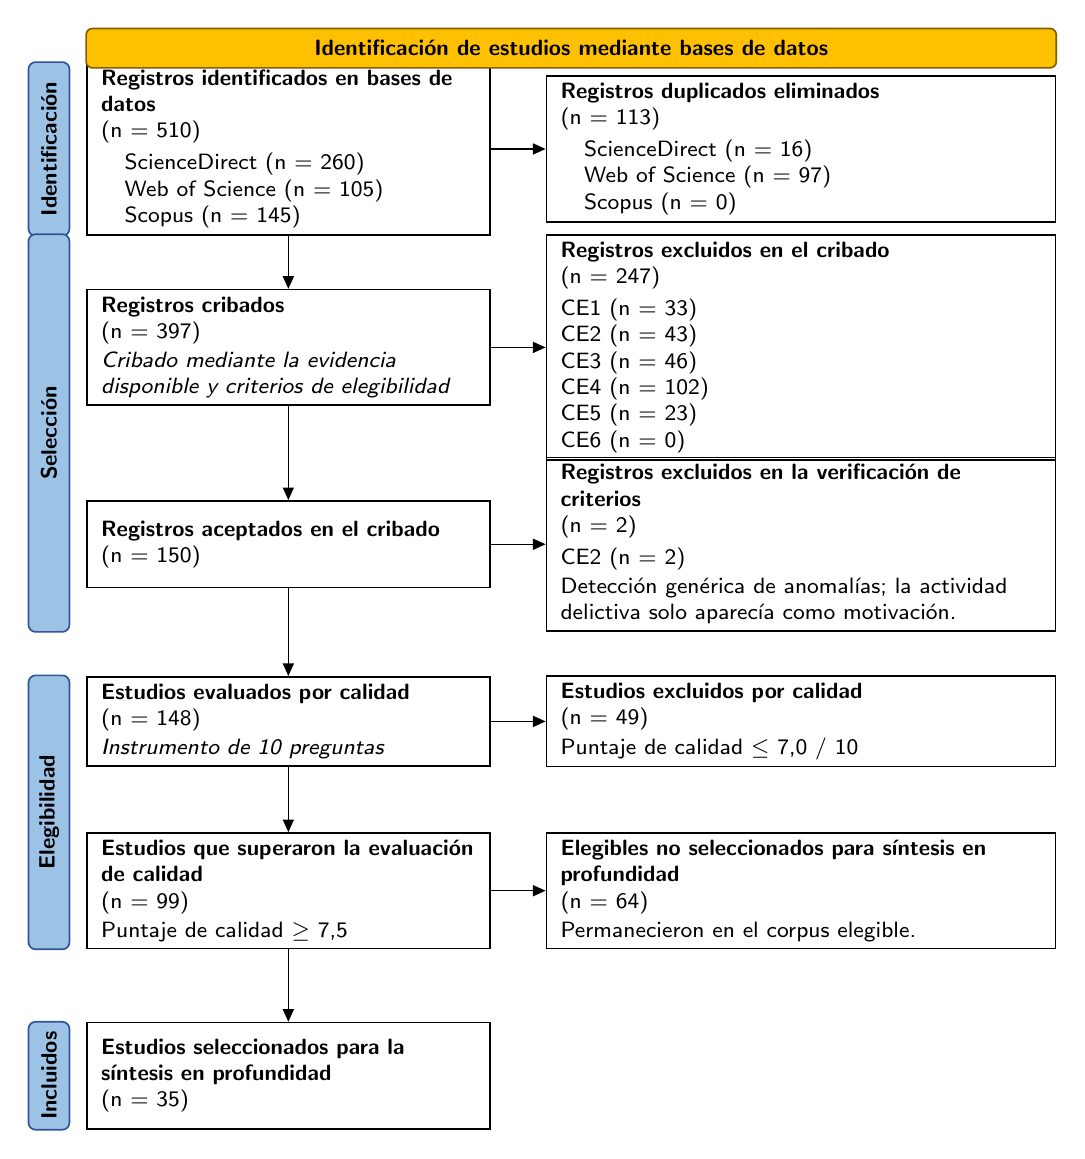
\begin{tikzpicture}[
    x=1cm, y=-1cm,
    font=\sffamily\footnotesize,
    execute at begin node={\hyphenpenalty=10000\exhyphenpenalty=10000},
    box/.style={draw, line width=0.6pt, rectangle, align=left,
                inner xsep=0.18cm, inner ysep=0.09cm},
    main/.style={box, text width=4.755cm, minimum height=1.10cm},
    side/.style={box, text width=6.105cm},
    flow/.style={-{Triangle[length=1.6mm,width=1.4mm]}, line width=0.5pt},
    band/.style={draw=bandline, fill=bandfill, line width=0.6pt,
                 rounded corners=0.9mm, inner sep=0pt},
  ]
  \definecolor{bandfill}{HTML}{9CC2E5}
  \definecolor{bandline}{HTML}{2F5496}
  \definecolor{headfill}{HTML}{FFC000}
  \definecolor{headline}{HTML}{7F5F00}

  % Ejes de las columnas (cm)
  \def\xl{3.30}
  \def\xr{9.81}

  % ====================== IDENTIFICACION =====================
  \node[main] (m1) at (\xl, 1.58) {%
    \textbf{Registros identificados en bases de datos}\\
    (n = 510)\\[2pt]
    \hspace*{1em}ScienceDirect (n = 260)\\
    \hspace*{1em}Web of Science (n = 105)\\
    \hspace*{1em}Scopus (n = 145)};
  \node[side, minimum height=1.66cm] (r1) at (\xr, 1.58) {%
    \textbf{Registros duplicados eliminados}\\
    (n = 113)\\[2pt]
    \hspace*{1em}ScienceDirect (n = 16)\\
    \hspace*{1em}Web of Science (n = 97)\\
    \hspace*{1em}Scopus (n = 0)};

  % ========================= SELECCION =======================
  \node[main] (m2) at (\xl, 4.10) {%
    \textbf{Registros cribados}\\
    (n = 397)\\[1pt]
    \textit{Cribado mediante la evidencia disponible y criterios de elegibilidad}};
  \node[side] (r2) at (\xr, 4.10) {%
    \textbf{Registros excluidos en el cribado}\\
    (n = 247)\\[2pt]
    CE1 (n = 33)\\
    CE2 (n = 43)\\
    CE3 (n = 46)\\
    CE4 (n = 102)\\
    CE5 (n = 23)\\
    CE6 (n = 0)};
  \node[main] (m3) at (\xl, 6.60) {%
    \textbf{Registros aceptados en el cribado}\\
    (n = 150)};
  \node[side] (r3) at (\xr, 6.60) {%
    \textbf{Registros excluidos en la verificación de criterios}\\
    (n = 2)\\[2pt]
    CE2 (n = 2)\\[1pt]
    Detección genérica de anomalías; la actividad delictiva solo aparecía como motivación.};

  % ======================== ELEGIBILIDAD =====================
  \node[main] (m4) at (\xl, 8.85) {%
    \textbf{Estudios evaluados por calidad}\\
    (n = 148)\\[1pt]
    \textit{Instrumento de 10 preguntas}};
  \node[side, minimum height=1.10cm] (r4) at (\xr, 8.85) {%
    \textbf{Estudios excluidos por calidad}\\
    (n = 49)\\[1pt]
    Puntaje de calidad $\leq$ 7,0 / 10};
  \node[main] (m5) at (\xl, 11.00) {%
    \textbf{Estudios que superaron la evaluación de calidad}\\
    (n = 99)\\[1pt]
    Puntaje de calidad $\geq$ 7,5};
  \node[side, minimum height=1.10cm] (r6) at (\xr, 11.00) {%
    \textbf{Elegibles no seleccionados para síntesis en profundidad}\\
    (n = 64)\\[1pt]
    Permanecieron en el corpus elegible.};

  % ========================= INCLUIDOS =======================
  \node[main, minimum height=1.35cm] (m6) at (\xl, 13.35) {%
    \textbf{Estudios seleccionados para la síntesis en profundidad}\\
    (n = 35)};

  % ========================= CABECERA ========================
  \node[draw=headline, fill=headfill, line width=0.6pt,
        rounded corners=0.8mm, inner sep=0pt,
        fit={(m1.west |- 0,0.05) (r1.east |- 0,0.55)}] (head) {};
  \node[font=\sffamily\footnotesize\bfseries] at (head.center)
    {Identificación de estudios mediante bases de datos};

  % ========================== FLECHAS ========================
  % Flujo principal vertical (borde inferior -> borde superior)
  \draw[flow] (m1.south) -- (m2.north);
  \draw[flow] (m2.south) -- (m3.north);
  \draw[flow] (m3.south) -- (m4.north);
  \draw[flow] (m4.south) -- (m5.north);
  \draw[flow] (m5.south) -- (m6.north);
  % Salidas laterales: desde el borde derecho de la caja principal
  \draw[flow] (m1.east) -- (r1.west |- m1.east);
  \draw[flow] (m2.east) -- (r2.west |- m2.east);
  \draw[flow] (m3.east) -- (r3.west |- m3.east);
  \draw[flow] (m4.east) -- (r4.west |- m4.east);
  \draw[flow] (m5.east) -- (r6.west |- m5.east);

  % ====================== BANDAS DE FASE =====================
  \def\bxa{0.00}\def\bxb{0.52}
  \newcommand{\phaseband}[4]{%
    \node[band, fit={(\bxa, 0 |- #1) (\bxb, 0 |- #2)}] (#3) {};
    \node[rotate=90, font=\sffamily\footnotesize\bfseries] at (#3.center) {#4};}
  \phaseband{m1.north}{m1.south}{p1}{Identificación}
  \phaseband{r2.north}{r3.south}{p2}{Selección}
  \phaseband{r4.north}{r6.south}{p3}{Elegibilidad}
  \phaseband{m6.north}{m6.south}{p4}{Incluidos}
\end{tikzpicture}

\caption{Flujo de identificación y selección de estudios inspirado en PRISMA 2020 \cite{page2021} y adaptado al proceso de revisión sistemática de Kitchenham y Charters \cite{kitchenham2007}. CE: criterio de exclusión (definiciones en la Tabla~\ref{tab:criterios})}\label{fig:prisma-argus}
\end{figure}

\FloatBarrier
\subsection{Evaluación de calidad}\label{subsec:calidad}

Los 148 estudios que superaron la selección se sometieron a una evaluación de calidad con un instrumento de diez preguntas (Tabla~\ref{tab:qa}). Las preguntas examinaron el contexto de aplicación, la descripción del conjunto de datos, la metodología de evaluación, las métricas reportadas, la declaración de limitaciones, la discusión frente a trabajos previos, el detalle necesario para la replicación, la descripción del modelo, la coherencia entre objetivo y evaluación y la comparación con al menos una línea base. Kitchenham y Charters recomiendan definir el instrumento de calidad en el protocolo y especificar el uso que se dará a sus resultados \cite{kitchenham2007}, y el empleo de listas de verificación para valorar estudios primarios cuenta con precedentes en revisiones sistemáticas de ingeniería de software \cite{dyba2008}. Cada pregunta se calificó como Sí (1), Parcialmente (0,5) o No (0), por lo que el puntaje máximo fue de 10 puntos. Se consideró que un estudio superaba la evaluación cuando obtenía al menos 7,5 puntos, y que no la superaba con 7,0 puntos o menos; como la escala avanzaba en pasos de 0,5, no existían puntajes intermedios entre ambos límites. Este umbral fue una decisión propia de la revisión: en Parsifal se configuró un punto de corte de 7,0 y solo los puntajes superiores a ese valor se consideraron aprobatorios. Con él, 99 estudios superaron la evaluación y 49 no la superaron; entre estos últimos, siete obtuvieron exactamente 7,0 puntos. En 45 de los 148 estudios se registró acceso limitado al texto completo; en esos casos, la valoración se realizó con la evidencia documental disponible y el acceso limitado no se utilizó como criterio de exclusión: tres de esos estudios superaron la evaluación y 42 no la superaron.

\begin{table}[h]
\hyphenpenalty=10000\exhyphenpenalty=10000
\caption{Instrumento de evaluación de calidad de los estudios}\label{tab:qa}
\begin{tabular}{@{}L{1.0cm}L{11.5cm}@{}}
\toprule
Código & Pregunta \\
\midrule
QA1 & ¿El estudio describe con suficiente detalle el contexto o escenario de aplicación en el que se desarrolla o evalúa el sistema? \\
QA2 & ¿El conjunto de datos utilizado está adecuadamente descrito en cuanto a origen, tamaño y características relevantes para la tarea evaluada? \\
QA3 & ¿La metodología de evaluación o validación está claramente descrita y es apropiada para el objetivo y la tarea del estudio? \\
QA4 & ¿El estudio reporta métricas cuantitativas de desempeño apropiadas para la tarea evaluada, ya sea detección, seguimiento u otra tarea relacionada? \\
QA5 & ¿El estudio declara limitaciones, amenazas a la validez o problemas de generalización de los resultados? \\
QA6 & ¿Los resultados se interpretan o discuten en relación con la literatura previa o con otros métodos, más allá de la mera presentación de resultados? \\
QA7 & ¿El estudio proporciona suficiente detalle metodológico y experimental para permitir, en principio, la reproducción o replicación del procedimiento realizado? \\
QA8 & ¿Se describe con suficiente detalle el modelo, algoritmo o arquitectura de Inteligencia Artificial utilizada, permitiendo comprender su funcionamiento? \\
QA9 & ¿El estudio define con claridad su objetivo o problema de investigación, y existe coherencia entre dicho objetivo, el método propuesto y la evaluación realizada? \\
QA10 & ¿El modelo o método propuesto se compara cuantitativamente con al menos un método, modelo o línea base relevante? \\
\bottomrule
\end{tabular}
\footnotetext{Escala: Sí = 1; Parcialmente = 0,5; No = 0; puntaje máximo = 10.}
\end{table}

\FloatBarrier
\subsection{Extracción de datos y selección para la síntesis}\label{subsec:extraccion}

La extracción de datos se aplicó a los 99 estudios que superaron la evaluación de calidad, mediante un formulario de 30 campos definido en Parsifal, en línea con la recomendación de diseñar los formularios de extracción para recoger la información necesaria para responder las preguntas de la revisión \cite{kitchenham2007}. Los campos registraron la identificación bibliográfica, el país o la ubicación del escenario, el conjunto de datos con su origen y características, el escenario de videovigilancia, la tarea principal y el evento de seguridad específico, la arquitectura o modelo de Inteligencia Artificial, el protocolo de evaluación, las métricas reportadas (exactitud, precisión, recall, F1-Score, mAP, AUC, latencia, FPS y otras métricas), la evidencia de procesamiento en tiempo real, la arquitectura de despliegue, la línea base de comparación, el hallazgo principal, las limitaciones declaradas por los autores y el puntaje de calidad. El formulario comprendió 2\,970 celdas ($99 \times 30$). La extracción sirvió para caracterizar los estudios y no se utilizó como criterio de exclusión.

Los 99 estudios que superaron la evaluación de calidad constituyeron el corpus elegible de la revisión y sustentaron los conteos y frecuencias globales de RQ1--RQ5. Después de la extracción, 35 de ellos se seleccionaron para una síntesis en profundidad mediante un muestreo intencional de máxima variación (\textit{purposeful maximum-variation sampling}), estrategia que, aplicada a la síntesis de investigaciones, consiste en identificar dimensiones clave de variación y elegir estudios que difieran entre sí a lo largo de ellas \cite{suri2011}. Las dimensiones consideradas fueron la tarea principal, la familia de modelos, la cobertura de RQ1--RQ5, los conjuntos de datos, el año de publicación y la evidencia de despliegue o de procesamiento en tiempo real. Además, se redujo la redundancia entre estudios con la misma tarea y familia de modelos y se mantuvieron representadas las familias poco frecuentes en el corpus. El puntaje de calidad y la disponibilidad del texto completo actuaron solo como criterios secundarios de desempate. La selección se basó en un juicio metodológico documentado a partir de los datos extraídos; no respondió a un algoritmo determinista, no estuvo preespecificada en el protocolo inicial y no consideró el desempeño reportado por los modelos. Muestreos intencionales de este tipo se han empleado en síntesis de evidencia para trabajar con un subconjunto de los estudios elegibles, manteniendo identificados los estudios que no se incorporaron al análisis \cite{ames2019}. Los 64 estudios restantes no se excluyeron de la revisión: superaron la evaluación de calidad, permanecieron en el corpus elegible y se consideraron en los conteos globales, aunque no formaron parte de la síntesis en profundidad. De este modo, los 99 estudios sustentaron los conteos globales y el subconjunto de 35 permitió realizar una síntesis más detallada conservando la diversidad del corpus. En la sección de resultados, el subconjunto de 35 estudios se denomina \textit{Reporting Core}.

Siguiendo la recomendación de reportar las amenazas a la validez en estudios secundarios \cite{ampatzoglou2019}, se identificaron las siguientes limitaciones metodológicas. La búsqueda se limitó a tres bases de datos y a los filtros de periodo, tipo documental, idioma (inglés en Web of Science y Scopus; ScienceDirect no ofrecía un filtro equivalente) y acceso abierto, por lo que pueden existir estudios pertinentes que no fueron recuperados; las diferencias de cobertura entre fuentes bibliográficas \cite{martin2021} hacen que esta restricción no sea despreciable. Además, la cadena no incluyó algunos términos registrados en el protocolo, entre ellos los de re-identificación, reconocimiento facial e identificación de personas, lo que pudo reducir la recuperación de estudios centrados en esas técnicas. No se aplicó búsqueda por bola de nieve hacia atrás o hacia adelante (\textit{snowballing}), técnica que permite recuperar estudios no capturados por las cadenas booleanas \cite{wohlin2014}. En los registros del protocolo y de la ejecución de la búsqueda no consta una evaluación de la sensibilidad de la estrategia frente a un conjunto de referencia de estudios relevantes conocidos (cuasi estándar de oro), por lo que no es posible estimar la proporción de estudios pertinentes efectivamente recuperada \cite{zhang2011}. Por último, la valoración de calidad de los estudios con acceso limitado al texto completo se apoyó únicamente en la evidencia documental disponible (subsección~\ref{subsec:calidad}).


% ============================================================
% 3. RESULTADOS
% ============================================================

\section{Resultados}\label{sec3}

Los resultados se organizaron en tres niveles. Primero, se presenta una síntesis
integral orientada a responder la pregunta general de investigación mediante los
estudios que conforman el \textit{Reporting Core}. Posteriormente, se desarrollan
las cinco preguntas específicas de investigación (RQ1--RQ5), considerando los
modelos de Inteligencia Artificial, los eventos de seguridad abordados, los
conjuntos de datos y escenarios utilizados, las métricas de evaluación y la
evidencia de implementación. Finalmente, se presentan los resultados del análisis
bibliométrico desarrollado a partir de los registros recuperados de Scopus.

El corpus final estuvo conformado por 99 estudios que superaron la evaluación de
calidad. Estos trabajos constituyen la base de los conteos y frecuencias globales.
Dentro de este conjunto se seleccionaron 35 estudios como \textit{Reporting Core},
los cuales fueron utilizados para profundizar la síntesis cualitativa y conservar
la trazabilidad de los principales hallazgos hacia publicaciones específicas.

Debido a que un mismo estudio puede utilizar diferentes arquitecturas, analizar
más de un evento de seguridad, emplear varios conjuntos de datos o reportar
múltiples métricas, algunas categorías fueron consideradas multietiqueta. Por ello,
los porcentajes correspondientes no necesariamente suman 100\,\%.

% ============================================================
% 3.1 PREGUNTA GENERAL
% ============================================================

\subsection{Síntesis de la pregunta general de investigación}
\label{subsec:rq_general}

La pregunta general buscó determinar qué modelos y técnicas de Inteligencia
Artificial han sido aplicados entre 2021 y 2026 en sistemas de videovigilancia
orientados a la detección de actividades delictivas y al seguimiento de personas
u objetos relacionados con eventos de seguridad, considerando también el desempeño
alcanzado y las evidencias de implementación reportadas.

Para responder esta pregunta de manera integrada, los estudios del
\textit{Reporting Core} fueron organizados según cuatro dimensiones principales:
la tecnología de Inteligencia Artificial empleada, el tipo de actividad o evento
de seguridad analizado, las capacidades de identificación o seguimiento y la
evidencia relacionada con evaluación e implementación. La
Tabla~\ref{tab:general_synthesis} resume esta información.

\begingroup
\footnotesize
\setlength{\tabcolsep}{2.5pt}
\renewcommand{\arraystretch}{1.12}

\begin{longtable}{@{}L{2.0cm}L{2.5cm}L{2.55cm}L{2.4cm}L{2.9cm}@{}}

\caption{Síntesis de los estudios del Reporting Core para la pregunta general de investigación}
\label{tab:general_synthesis}\\

\toprule
\textbf{Referencia} &
\textbf{Modelos y técnicas de IA} &
\textbf{Actividad o evento de seguridad} &
\textbf{Identificación y seguimiento} &
\textbf{Desempeño e implementación} \\
\midrule
\endfirsthead

\multicolumn{5}{c}
{{\tablename\ \thetable{} -- continuación}}\\

\toprule
\textbf{Referencia} &
\textbf{Modelos y técnicas de IA} &
\textbf{Actividad o evento de seguridad} &
\textbf{Identificación y seguimiento} &
\textbf{Desempeño e implementación} \\
\midrule
\endhead

\midrule
\multicolumn{5}{r}{Continúa en la página siguiente}\\
\endfoot

\bottomrule
\endlastfoot

\citet{munoz2025} &
YOLO / detector de objetos &
Armas de fuego &
No reportado &
mAP; tiempo real declarado; despliegue descrito \\

\citet{ciampi2024} &
CNN 2D &
Violencia / agresión física &
No reportado &
Evaluación en SCF, RLVS y RWF-2000 \\

\citet{singhal2026} &
LSTM y 3D-CNN &
Actividades delictivas y armas &
No reportado &
Accuracy, Precision, Recall, F1 y AUC \\

\citet{bhavani2025} &
Esqueleto / pose &
Violencia y actividades delictivas &
Seguimiento de movimiento &
Accuracy, Precision, Recall y F1 \\

\citet{janbi2024} &
GCN, ensemble y pose &
Violencia &
Seguimiento de personas y esqueleto &
Evaluación en RLVS y NTU-Violence \\

\citet{shah2023} &
Enfoque inspirado en computación cuántica &
Armas &
No reportado &
Tiempo real declarado \\

\citet{ciampi2022} &
Transformer, LSTM y 3D-CNN &
Violencia &
No reportado &
Evaluación en múltiples benchmarks \\

\citet{fierrosilva2026} &
YOLO / detector de objetos &
Armas &
Seguimiento multicámara &
Tiempo real demostrado; despliegue descrito \\

\citet{huszar2023} &
3D-CNN &
Violencia &
No reportado &
Evaluación sobre múltiples datasets \\

\citet{fathy2022} &
YOLO / detector de objetos &
Armas &
No reportado &
Tiempo real demostrado; despliegue descrito \\

\citet{muriithi2024} &
Esqueleto / pose &
Armas &
Seguimiento de personas y movimiento &
Evaluación experimental \\

\citet{shin2025} &
Transformer y 3D-CNN &
Comportamiento anómalo &
No reportado &
Evaluación en XD-Violence, ShanghaiTech y UCF-Crime \\

\citet{pangavhane2025} &
LSTM &
Comportamiento anómalo &
No reportado &
Evaluación en KTH Human Motion \\

\citet{dalal2024} &
YOLO / detector de objetos &
Personas u objetos de interés &
No reportado &
Evaluación en dataset basado en Roboflow \\

\citet{ingle2022} &
CNN 2D &
Armas &
No reportado &
Tiempo real demostrado; despliegue descrito \\

\citet{saleem2022} &
CNN 2D &
Comportamiento anómalo &
No reportado &
Tiempo real demostrado; despliegue descrito \\

\citet{azzakhnini2025} &
LSTM &
Violencia &
No reportado &
Tiempo real demostrado \\

\citet{g2025} &
GCN &
Violencia &
No reportado &
Tiempo real declarado \\

\citet{sernani2021} &
3D-CNN &
Violencia &
No reportado &
Evaluación experimental \\

\citet{salman2026} &
GRU &
Violencia &
No reportado &
Tiempo real demostrado \\

\citet{shah2025} &
Enfoque inspirado en computación cuántica &
Armas &
No reportado &
Tiempo real declarado \\

\citet{silva2026} &
YOLO / detector de objetos &
Armas &
No reportado &
Tiempo real demostrado; despliegue descrito \\

\citet{park2024} &
3D-CNN &
Violencia &
No reportado &
Tiempo real demostrado \\

\citet{pereatrigo2023} &
CNN 2D &
Armas &
No reportado &
Tiempo real demostrado; despliegue descrito \\

\citet{donia2023} &
ML clásico e ingeniería de características &
Violencia &
No reportado &
Evaluación experimental \\

\citet{azam2026} &
LSTM &
Comportamiento anómalo &
No reportado &
Tiempo real demostrado; despliegue descrito \\

\citet{singh2026} &
Autoencoder / GAN &
Armas &
No reportado &
Tiempo real demostrado \\

\citet{jokhio2024} &
Ensemble &
Comportamiento anómalo &
No reportado &
Tiempo real declarado \\

\citet{sandhya2022} &
Autoencoder / GAN &
Identificación de personas &
Reconocimiento facial &
Evaluación experimental \\

\citet{matei2025} &
CNN 2D &
Actividades delictivas &
Seguimiento de personas y esquelético &
Evaluación experimental \\

\citet{lin2025} &
CNN 2D &
Personas u objetos de interés &
No reportado &
Arquitectura de despliegue descrita \\

\citet{garciacobo2023} &
Esqueleto / pose &
Violencia &
Seguimiento de personas y esqueleto &
Tiempo real demostrado \\

\citet{tonmoy2025} &
Aprendizaje federado &
Violencia y armas &
No reportado &
Tiempo real declarado \\

\citet{gao2026} &
GRU y enfoque causal &
Comportamiento anómalo &
No reportado &
Tiempo real demostrado \\

\citet{leyva2024} &
GCN y modelo bayesiano &
Comportamiento anómalo &
Seguimiento de personas, objetos y multiobjeto &
Evaluación en múltiples datasets \\

\end{longtable}

\normalsize
\setlength{\tabcolsep}{6pt}
\endgroup

De manera global, la síntesis muestra un predominio de modelos de aprendizaje
profundo orientados a la detección de violencia, armas y comportamiento anómalo.
Las arquitecturas CNN, los detectores basados en YOLO y los modelos
espacio-temporales aparecen de forma recurrente, mientras que las funciones de
identificación y seguimiento presentan una presencia comparativamente menor.

También se observa que una parte importante de las evaluaciones se realiza sobre
datasets públicos y benchmarks. Aunque varios trabajos reportan o declaran
procesamiento en tiempo real, la documentación de arquitecturas completas de
despliegue es menos frecuente. Estos patrones generales se analizan de manera
específica en las preguntas RQ1--RQ5.

\subsection{Desarrollo de las preguntas de investigación}
\label{subsec:rq_development}

A partir de los patrones identificados en la síntesis general, las cinco preguntas
específicas permitieron examinar con mayor detalle las dimensiones tecnológicas,
experimentales y operativas de los sistemas de videovigilancia inteligente. Cada
pregunta se analizó utilizando los 99 estudios del corpus final para los conteos
globales y los trabajos del \textit{Reporting Core} para ejemplificar los hallazgos
más representativos.

\subsubsection{RQ1: Modelos, algoritmos y arquitecturas de Inteligencia Artificial}
\label{subsec:rq1_results}

La evidencia muestra una concentración en arquitecturas de aprendizaje profundo,
aunque con diferencias según la tarea abordada. Las CNN 2D fueron identificadas
en 25 de los 99 estudios (25,3\,\%), constituyendo la familia más frecuente.
Los detectores de objetos basados principalmente en YOLO aparecieron en 20 estudios
(20,2\,\%), seguidos por arquitecturas LSTM o recurrentes en 16 (16,2\,\%) y
3D-CNN en 13 (13,1\,\%). Los mecanismos de atención y Transformer estuvieron
presentes en nueve estudios (9,1\,\%), mientras que los enfoques basados en
esqueleto o pose y GCN aparecieron en siete (7,1\,\%) y seis (6,1\,\%),
respectivamente.

Los detectores YOLO se utilizaron predominantemente en tareas de localización de
armas y objetos de riesgo, mientras que la detección de violencia presentó una
mayor diversidad arquitectónica, incluyendo CNN 2D, 3D-CNN, LSTM, GRU,
Transformers y modelos basados en grafos. También se identificaron aproximaciones
menos frecuentes basadas en aprendizaje federado, autoencoders, métodos bayesianos,
modelos causales y técnicas inspiradas en computación cuántica.

\begingroup
\small
\setlength{\tabcolsep}{4pt}
\renewcommand{\arraystretch}{1.15}
\begin{longtable}{@{}L{3.2cm}L{5.0cm}L{4.1cm}@{}}
\caption{Resultados para RQ1: principales familias de modelos y estudios representados en el Reporting Core}
\label{tab:rq1_results}\\
\toprule
\textbf{Modelo / arquitectura} & \textbf{Referencias representativas} & \textbf{Aplicación predominante} \\
\midrule
\endfirsthead
\multicolumn{3}{c}{\tablename\ \thetable{} -- continuación}\\
\toprule
\textbf{Modelo / arquitectura} & \textbf{Referencias representativas} & \textbf{Aplicación predominante} \\
\midrule
\endhead
\midrule
\multicolumn{3}{r}{Continúa en la página siguiente}\\
\endfoot
\bottomrule
\endlastfoot
CNN 2D (25/99) & \citet{ciampi2024}; \citet{ingle2022}; \citet{saleem2022}; \citet{pereatrigo2023} & Violencia, anomalías y armas \\
YOLO / detectores de objetos (20/99) & \citet{munoz2025}; \citet{fierrosilva2026}; \citet{fathy2022}; \citet{dalal2024} & Detección y localización de armas u objetos \\
LSTM / arquitecturas recurrentes (16/99) & \citet{singhal2026}; \citet{ciampi2022}; \citet{pangavhane2025}; \citet{azzakhnini2025} & Análisis temporal de secuencias \\
3D-CNN (13/99) & \citet{singhal2026}; \citet{ciampi2022}; \citet{huszar2023}; \citet{shin2025} & Reconocimiento espacio-temporal de acciones \\
Transformer / mecanismos de atención (9/99) & \citet{ciampi2022}; \citet{shin2025} & Representación de dependencias espacio-temporales \\
Esqueleto / pose (7/99) & \citet{bhavani2025}; \citet{janbi2024}; \citet{muriithi2024}; \citet{garciacobo2023} & Análisis del movimiento corporal \\
GCN / modelos basados en grafos (6/99) & \citet{janbi2024}; \citet{g2025}; \citet{leyva2024} & Relaciones estructurales y comportamiento \\
\end{longtable}
\endgroup

La distribución indica que no existe una única arquitectura empleada de forma
transversal para todas las funciones de videovigilancia. La elección del modelo se
encuentra estrechamente asociada con la naturaleza de la tarea: la localización de
objetos utiliza con mayor frecuencia detectores de una etapa, mientras que el
reconocimiento de acciones incorpora modelos capaces de representar relaciones
espacio-temporales.


% ============================================================
% 3.2.2 RQ2
% ============================================================

\subsubsection{RQ2: Actividades delictivas, eventos de seguridad y capacidades de seguimiento}
\label{subsec:rq2_results}

La violencia o agresión física fue el evento con mayor presencia en el corpus,
identificado en 52 de los 99 estudios (52,5\,\%). La detección de armas de fuego
ocupó el segundo lugar, con 29 estudios (29,3\,\%). También se identificaron
eventos delictivos o anómalos múltiples en 15 trabajos (15,2\,\%),
comportamiento sospechoso o anomalía general en 13 (13,1\,\%), armas blancas
en 11 (11,1\,\%) y robo o hurto en 10 (10,1\,\%).

\begingroup
\small
\setlength{\tabcolsep}{4pt}
\renewcommand{\arraystretch}{1.15}
\begin{longtable}{@{}L{3.2cm}L{5.0cm}L{4.1cm}@{}}
\caption{Resultados para RQ2: eventos de seguridad y capacidades de seguimiento}
\label{tab:rq2_results}\\
\toprule
\textbf{Evento / capacidad} & \textbf{Referencias representativas} & \textbf{Función} \\
\midrule
\endfirsthead
\multicolumn{3}{c}{\tablename\ \thetable{} -- continuación}\\
\toprule
\textbf{Evento / capacidad} & \textbf{Referencias representativas} & \textbf{Función} \\
\midrule
\endhead
\midrule
\multicolumn{3}{r}{Continúa en la página siguiente}\\
\endfoot
\bottomrule
\endlastfoot
Violencia / agresión física (52/99) & \citet{ciampi2024}; \citet{bhavani2025}; \citet{janbi2024}; \citet{ciampi2022} & Reconocer episodios de violencia o agresión \\
Arma de fuego (29/99) & \citet{munoz2025}; \citet{singhal2026}; \citet{bhavani2025}; \citet{shah2023} & Detectar y localizar armas de fuego \\
Eventos delictivos / anómalos múltiples (15/99) & \citet{singhal2026}; \citet{shin2025}; \citet{saleem2022}; \citet{g2025} & Reconocer varias categorías de eventos \\
Comportamiento sospechoso / anomalía general (13/99) & \citet{shin2025}; \citet{pangavhane2025}; \citet{saleem2022}; \citet{azam2026} & Detectar comportamientos sospechosos o anómalos \\
Arma blanca (11/99) & \citet{shah2023}; \citet{fierrosilva2026}; \citet{fathy2022}; \citet{ingle2022} & Detectar armas blancas \\
Robo / hurto (10/99) & \citet{ciampi2022}; \citet{saleem2022}; \citet{jokhio2024} & Reconocer eventos de robo o hurto \\
Seguimiento general (13/99) & \citet{bhavani2025}; \citet{janbi2024}; \citet{fierrosilva2026}; \citet{muriithi2024} & Mantener la trayectoria de entidades entre fotogramas \\
Seguimiento de personas (8/99) & \citet{janbi2024}; \citet{muriithi2024}; \citet{matei2025}; \citet{garciacobo2023} & Seguir personas dentro de una secuencia \\
Seguimiento multicámara (1/99) & \citet{fierrosilva2026} & Relacionar el seguimiento entre cámaras \\
Identificación / reconocimiento de personas & \citet{sandhya2022} & Reconocer la identidad de una persona \\
Re-identificación explícitamente evaluada (0/99) & No se identificaron estudios en el corpus final & Asociar identidades entre observaciones; sin evaluación explícita en este corpus \\
\end{longtable}
\endgroup

En conjunto, 18 de los 99 estudios incorporaron alguna capacidad de seguimiento o
identificación. El seguimiento apareció mayoritariamente como componente complementario
a la tarea principal y no como objetivo experimental independiente. Asimismo, no se
identificaron estudios que evaluaran explícitamente re-identificación de personas con
métricas especializadas. Este resultado describe exclusivamente el corpus recuperado
por la estrategia de búsqueda y no implica ausencia de trabajos sobre
\textit{person re-identification} en la literatura general.


% ============================================================
% 3.2.3 RQ3
% ============================================================

\subsubsection{RQ3: Conjuntos de datos y escenarios de videovigilancia}
\label{subsec:rq3_results}

Los experimentos se concentraron en un número limitado de conjuntos de datos.
Hockey Fight fue utilizado en 19 estudios (19,2\,\%), UCF-Crime en 15
(15,2\,\%), RWF-2000 en 14 (14,1\,\%), Movie Fights en 11 (11,1\,\%)
y RLVS en 10 (10,1\,\%). En cuanto al origen, 56 estudios utilizaron
principalmente datos públicos o benchmarks, 24 combinaron datos públicos y propios,
y 19 emplearon principalmente conjuntos propios o privados.

\begingroup
\small
\setlength{\tabcolsep}{4pt}
\renewcommand{\arraystretch}{1.15}
\begin{longtable}{@{}L{3.2cm}L{5.0cm}L{4.1cm}@{}}
\caption{Resultados para RQ3: principales conjuntos de datos identificados}
\label{tab:rq3_results}\\
\toprule
\textbf{Dataset / protocolo} & \textbf{Referencias representativas} & \textbf{Aplicación} \\
\midrule
\endfirsthead
\multicolumn{3}{c}{\tablename\ \thetable{} -- continuación}\\
\toprule
\textbf{Dataset / protocolo} & \textbf{Referencias representativas} & \textbf{Aplicación} \\
\midrule
\endhead
\midrule
\multicolumn{3}{r}{Continúa en la página siguiente}\\
\endfoot
\bottomrule
\endlastfoot
Hockey Fight (19/99) & \citet{huszar2023}; \citet{azzakhnini2025}; \citet{salman2026}; \citet{donia2023} & Detección de violencia \\
UCF-Crime (15/99) & \citet{singhal2026}; \citet{shin2025}; \citet{saleem2022}; \citet{gao2026} & Detección de actividades delictivas y anomalías \\
RWF-2000 (14/99) & \citet{ciampi2024}; \citet{ciampi2022}; \citet{huszar2023}; \citet{azzakhnini2025} & Detección de violencia en video \\
Movie Fights (11/99) & \citet{huszar2023}; \citet{azam2026} & Reconocimiento de peleas y violencia \\
RLVS (10/99) & \citet{ciampi2024}; \citet{janbi2024}; \citet{ciampi2022}; \citet{huszar2023} & Detección de violencia \\
Sohas Weapon Detection & \citet{fierrosilva2026}; \citet{fathy2022}; \citet{silva2026} & Detección de armas \\
Evaluación \textit{cross-dataset} explícita (3/99) & \citet{ciampi2024}; \citet{ciampi2022}; \citet{huszar2023} & Evaluación de generalización entre conjuntos de datos \\
\end{longtable}
\endgroup

Cuarenta y dos estudios evaluaron sus modelos empleando dos o más conjuntos de
datos; sin embargo, únicamente tres realizaron una evaluación
\textit{cross-dataset} explícita. Adicionalmente, el escenario de videovigilancia
no fue especificado en 38 estudios y otros 18 lo describieron únicamente como
CCTV genérico.

\begingroup
\small
\setlength{\tabcolsep}{4pt}
\renewcommand{\arraystretch}{1.15}
\begin{longtable}{@{}L{9.0cm}L{3.6cm}@{}}
\caption{Escenarios de videovigilancia reportados con mayor frecuencia}
\label{tab:rq3_scenarios}\\
\toprule
\textbf{Tipo de escenario} & \textbf{Número de estudios} \\
\midrule
\endfirsthead
\multicolumn{2}{c}{\tablename\ \thetable{} -- continuación}\\
\toprule
\textbf{Tipo de escenario} & \textbf{Número de estudios} \\
\midrule
\endhead
\midrule
\multicolumn{2}{r}{Continúa en la página siguiente}\\
\endfoot
\bottomrule
\endlastfoot
No reportado & 38 \\
CCTV genérico & 18 \\
Interiores / hogar & 6 \\
Transporte público / estaciones & 5 \\
Espacios públicos & 5 \\
\end{longtable}
\endgroup

La Tabla~\ref{tab:rq3_scenarios} presenta las categorías más frecuentes;
no constituye una distribución exhaustiva de los 99 estudios.

Entre los escenarios explícitos se identificaron entornos interiores, transporte
público o estaciones y espacios públicos. Solo dos estudios documentaron de forma
explícita captura u operación en un entorno real confirmado. El país o ubicación
del escenario fue reportado únicamente en 28 de los 99 trabajos, lo que limita
la interpretación de la capacidad de generalización geográfica de los modelos.


% ============================================================
% 3.2.4 RQ4
% ============================================================

\subsubsection{RQ4: Métricas y niveles de desempeño}
\label{subsec:rq4_results}

La evaluación del desempeño presentó una marcada heterogeneidad entre los estudios.
Accuracy fue reportada en 60 estudios (60,6\,\%), F1-Score en 30 (30,3\,\%),
Precision y Recall en 28 estudios cada una (28,3\,\%), AUC en 16 (16,2\,\%)
y mAP en 14 (14,1\,\%). Respecto de la eficiencia computacional, 30 estudios
reportaron latencia y 15 informaron FPS.

\begingroup
\small
\setlength{\tabcolsep}{4pt}
\renewcommand{\arraystretch}{1.15}
\begin{longtable}{@{}L{3.2cm}L{5.0cm}L{4.1cm}@{}}
\caption{Resultados para RQ4: métricas utilizadas para evaluar los modelos}
\label{tab:rq4_results}\\
\toprule
\textbf{Métrica} & \textbf{Referencias representativas} & \textbf{Función} \\
\midrule
\endfirsthead
\multicolumn{3}{c}{\tablename\ \thetable{} -- continuación}\\
\toprule
\textbf{Métrica} & \textbf{Referencias representativas} & \textbf{Función} \\
\midrule
\endhead
\midrule
\multicolumn{3}{r}{Continúa en la página siguiente}\\
\endfoot
\bottomrule
\endlastfoot
Accuracy (60/99) & \citet{singhal2026}; \citet{bhavani2025}; \citet{janbi2024}; \citet{muriithi2024} & Proporción de clasificaciones correctas \\
F1-Score (30/99) & \citet{singhal2026}; \citet{bhavani2025}; \citet{ingle2022}; \citet{g2025} & Equilibrio entre Precision y Recall \\
Precision (28/99) & \citet{singhal2026}; \citet{bhavani2025}; \citet{fathy2022}; \citet{muriithi2024} & Proporción de positivos predichos que son correctos \\
Recall (28/99) & \citet{singhal2026}; \citet{bhavani2025}; \citet{fathy2022}; \citet{muriithi2024} & Proporción de positivos reales recuperados \\
AUC (16/99) & \citet{singhal2026}; \citet{shin2025}; \citet{sernani2021}; \citet{salman2026} & Capacidad discriminativa mediante el área bajo la curva \\
mAP (14/99) & \citet{munoz2025}; \citet{fathy2022}; \citet{dalal2024}; \citet{ingle2022} & Precisión media de detección de objetos \\
FPS (15/99) & Conteo agregado del corpus & Velocidad: fotogramas procesados por segundo \\
Latencia (30/99) & Conteo agregado del corpus & Tiempo de respuesta del procesamiento \\
\end{longtable}
\endgroup

Los conteos de FPS y latencia proceden de la síntesis agregada; el reporte
no individualiza sus referencias en esa tabla. Su interpretación requiere
considerar el hardware y las condiciones de medición.


Debido a las diferencias entre tareas, datasets, particiones experimentales,
protocolos de evaluación y escalas de las métricas, no se calculó un promedio global
de desempeño ni se estableció una clasificación general de los modelos.

No se identificaron grupos con comparabilidad metodológica alta. Se encontraron
cuatro grupos con comparabilidad moderada: SCVD para detección de violencia mediante
Accuracy, con resultados entre 93,5 y 96,15; Sohas Weapon Detection para detección
de armas mediante mAP, con valores entre 0,88 y 0,954; y UCF-Crime para
comportamiento anómalo mediante Accuracy, con valores entre 82,22 y 100, y mediante
F1-Score, con valores entre 99,89 y 100. Estos intervalos describen los resultados
reportados en condiciones relativamente semejantes, pero no permiten declarar un
modelo ganador general.

No se identificó el uso de métricas especializadas de seguimiento o
re-identificación como MOTA, MOTP, IDF1, HOTA, Rank-1, Rank-5, CMC o TAR.
Por tanto, los componentes de seguimiento encontrados fueron evaluados principalmente
mediante métricas generales de detección o clasificación.


% ============================================================
% 3.2.5 RQ5
% ============================================================

\subsubsection{RQ5: Procesamiento en tiempo real, despliegue y limitaciones}
\label{subsec:rq5_results}

Treinta y uno de los 99 estudios (31,3\,\%) presentaron evidencia experimental de
procesamiento en tiempo real y 27 (27,3\,\%) lo declararon sin una demostración
equivalente. Un estudio señaló explícitamente que no operaba en tiempo real y en
40 trabajos (40,4\,\%) esta característica no fue reportada.

Solo 21 estudios (21,2\,\%) describieron explícitamente una arquitectura de
despliegue, mientras que 78 (78,8\,\%) no proporcionaron esta información.

\begingroup
\small
\setlength{\tabcolsep}{4pt}
\renewcommand{\arraystretch}{1.15}
\begin{longtable}{@{}L{3.2cm}L{5.0cm}L{4.1cm}@{}}
\caption{Resultados para RQ5: evidencia de tiempo real y despliegue}
\label{tab:rq5_results}\\
\toprule
\textbf{Aspecto de implementación} & \textbf{Referencias representativas} & \textbf{Evidencia reportada} \\
\midrule
\endfirsthead
\multicolumn{3}{c}{\tablename\ \thetable{} -- continuación}\\
\toprule
\textbf{Aspecto de implementación} & \textbf{Referencias representativas} & \textbf{Evidencia reportada} \\
\midrule
\endhead
\midrule
\multicolumn{3}{r}{Continúa en la página siguiente}\\
\endfoot
\bottomrule
\endlastfoot
Tiempo real demostrado (31/99) & \citet{fierrosilva2026}; \citet{fathy2022}; \citet{ingle2022}; \citet{saleem2022} & Evidencia experimental de velocidad de procesamiento \\
Tiempo real declarado (27/99) & \citet{munoz2025}; \citet{shah2023}; \citet{g2025}; \citet{shah2025} & Afirmación de tiempo real sin demostración equivalente \\
Arquitectura de despliegue descrita (21/99) & \citet{munoz2025}; \citet{fierrosilva2026}; \citet{fathy2022}; \citet{ingle2022} & Descripción de componentes y organización del despliegue \\
\end{longtable}
\endgroup

Según el nivel de evidencia documentado en el corpus completo, siete estudios
presentaron un prototipo demostrado, 14 describieron una arquitectura propuesta,
26 reportaron únicamente el hardware utilizado durante la evaluación y 52 no
proporcionaron evidencia suficiente sobre despliegue. Ningún estudio documentó
una operación sostenida en producción.

Las plataformas identificadas con mayor frecuencia fueron dispositivos
\textit{edge} genéricos (13/99), NVIDIA Jetson (8/99) y Raspberry Pi (5/99).
Asimismo, 75 estudios declararon al menos una limitación. Las más frecuentes fueron
oclusión (16/99), falsos positivos o negativos (16/99), variaciones de iluminación
(13/99), baja diversidad de los conjuntos de datos (10/99), escenas complejas o
concurridas (9/99) y generalización limitada entre datasets (7/99).

\begingroup
\small
\setlength{\tabcolsep}{4pt}
\renewcommand{\arraystretch}{1.15}
\begin{longtable}{@{}L{9.0cm}L{3.6cm}@{}}
\caption{Limitaciones declaradas con mayor frecuencia en el corpus}
\label{tab:rq5_limitations}\\
\toprule
\textbf{Limitación} & \textbf{Frecuencia (N=99)} \\
\midrule
\endfirsthead
\multicolumn{2}{c}{\tablename\ \thetable{} -- continuación}\\
\toprule
\textbf{Limitación} & \textbf{Frecuencia (N=99)} \\
\midrule
\endhead
\midrule
\multicolumn{2}{r}{Continúa en la página siguiente}\\
\endfoot
\bottomrule
\endlastfoot
Oclusión & 16 \\
Falsos positivos o negativos & 16 \\
Variaciones de iluminación & 13 \\
Baja diversidad de los conjuntos de datos & 10 \\
Escenas complejas o concurridas & 9 \\
Generalización limitada entre datasets & 7 \\
\end{longtable}
\endgroup

Las limitaciones son multietiqueta: un estudio puede declarar más de una.

Un hallazgo adicional es que 25 de los 78 estudios que no describieron una arquitectura
de despliegue afirmaron procesamiento en tiempo real. En estos casos, la evidencia
correspondió principalmente a mediciones experimentales de velocidad o latencia y no
a una descripción completa de operación dentro de una infraestructura real de
videovigilancia.


% ============================================================
% 3.3 ANÁLISIS BIBLIOMÉTRICO
% ============================================================

\subsection{Resultados del análisis bibliométrico}
\label{subsec:bibliometric_results}

Como complemento de la revisión sistemática, se realizó un análisis bibliométrico
sobre los 145 registros recuperados de Scopus mediante el paquete
\textit{Bibliometrix}. Este conjunto se utilizó exclusivamente para caracterizar la
evolución temporal de la producción científica, la productividad de autores, revistas,
instituciones y países, las redes de colaboración y las estructuras intelectual y
conceptual del campo.

Los resultados bibliométricos se interpretan de manera independiente de los conteos
de la revisión sistemática. Mientras que la síntesis de RQ1--RQ5 utiliza el corpus
final elegible de 99 estudios, el análisis bibliométrico emplea los 145 documentos
correspondientes a Scopus.


% ------------------------------------------------------------
% BQ
% ------------------------------------------------------------

\subsubsection{BQ: Evolución de la producción científica y de las citas}
\label{subsubsec:bq}

La producción científica presentó una tendencia creciente entre 2021 y 2025.
El número de publicaciones pasó de 13 documentos en 2021 a 16 en 2022,
21 en 2023, 26 en 2024 y alcanzó su valor máximo con 40 publicaciones en 2025.
Para 2026 se recuperaron 29 documentos; sin embargo, debido a que la búsqueda se
realizó antes de finalizar dicho año, este valor no representa una producción anual
completa.

La tendencia de citación presentó un comportamiento diferente. Los documentos
publicados en 2021 y 2022 registraron los mayores promedios de citación, con
52,38 y 53,63 citas por publicación, respectivamente. Posteriormente, el promedio
disminuyó a 25,76 en 2023, 13,19 en 2024, 4,80 en 2025 y 0,38 en 2026.
Esta reducción debe interpretarse considerando el menor tiempo disponible para que
las publicaciones recientes acumulen citas.

\begin{table}[htbp]
\caption{Producción científica y citas medias por año en el corpus bibliométrico}
\label{tab:bq_annual}
\centering
\small
\begin{tabular}{@{}lrr@{}}
\toprule
\textbf{Año} & \textbf{Documentos} & \textbf{Citas medias} \\
\midrule
2021 & 13 & 52,38 \\
2022 & 16 & 53,63 \\
2023 & 21 & 25,76 \\
2024 & 26 & 13,19 \\
2025 & 40 & 4,80 \\
2026$^{a}$ & 29 & 0,38 \\
\bottomrule
\end{tabular}

\begin{flushleft}
\footnotesize $^{a}$ Año incompleto al momento de recuperar los registros.
\end{flushleft}
\end{table}


% ------------------------------------------------------------
% AB1
% ------------------------------------------------------------

\subsubsection{AB1: Productividad e influencia científica}
\label{subsubsec:ab1}

El análisis identificó 555 autores diferentes. La producción presentó una elevada
dispersión, ya que 521 autores participaron en un solo documento, mientras que
únicamente un grupo reducido apareció de manera recurrente en varias publicaciones.
Juan A. Álvarez-García registró cinco documentos en el corpus, seguido por
Oscar Deniz con cuatro. Fernando J. Rendón-Segador, Jesús Ruiz-Santaquiteria
y José L. Salazar-González registraron tres documentos cada uno.

Entre las fuentes de publicación, \textit{Sensors} presentó el mayor número de
documentos (13), seguida por \textit{IEEE Access} (9) y
\textit{Scientific Reports} (8). A nivel institucional, Princess Nourah Bint
Abdulrahman University y Universidad de Sevilla estuvieron asociadas a cinco
documentos cada una, seguidas por Islamia College Peshawar con cuatro.

En la dimensión geográfica, India presentó la mayor frecuencia de participación
(30 documentos), seguida por Pakistán (21), Arabia Saudita (20), Corea del Sur
(16), China (16), España (12), Egipto (10) e Italia (8).

\begin{table*}[htbp]
\caption{Principales actores identificados mediante el análisis bibliométrico}
\label{tab:ab1_productivity}
\centering
\small
\renewcommand{\arraystretch}{1.12}
\begin{tabular}{@{}L{2.5cm}L{7.2cm}r@{}}
\toprule
\textbf{Dimensión} & \textbf{Entidad} & \textbf{Documentos} \\
\midrule
Autor & Álvarez-García, J.A. & 5 \\
Autor & Deniz, O. & 4 \\
Autor & Rendón-Segador, F.J. & 3 \\
Autor & Ruiz-Santaquiteria, J. & 3 \\
Autor & Salazar-González, J.L. & 3 \\
\midrule
Fuente & \textit{Sensors} & 13 \\
Fuente & \textit{IEEE Access} & 9 \\
Fuente & \textit{Scientific Reports} & 8 \\
Fuente & \textit{Computers, Materials and Continua} & 5 \\
Fuente & \textit{PeerJ Computer Science} & 4 \\
\midrule
Institución & Princess Nourah Bint Abdulrahman University & 5 \\
Institución & Universidad de Sevilla & 5 \\
Institución & Islamia College Peshawar & 4 \\
Institución & King Saud University & 3 \\
Institución & University of Jeddah & 3 \\
\midrule
País & India & 30 \\
País & Pakistán & 21 \\
País & Arabia Saudita & 20 \\
País & Corea del Sur & 16 \\
País & China & 16 \\
\bottomrule
\end{tabular}
\end{table*}

El diagrama de tres campos complementa esta caracterización al representar las
relaciones entre diferentes componentes bibliográficos del corpus. Los flujos
permiten observar cómo autores, fuentes y conceptos se vinculan alrededor de los
principales temas de investigación.

\begin{figure*}[htbp]
\centering
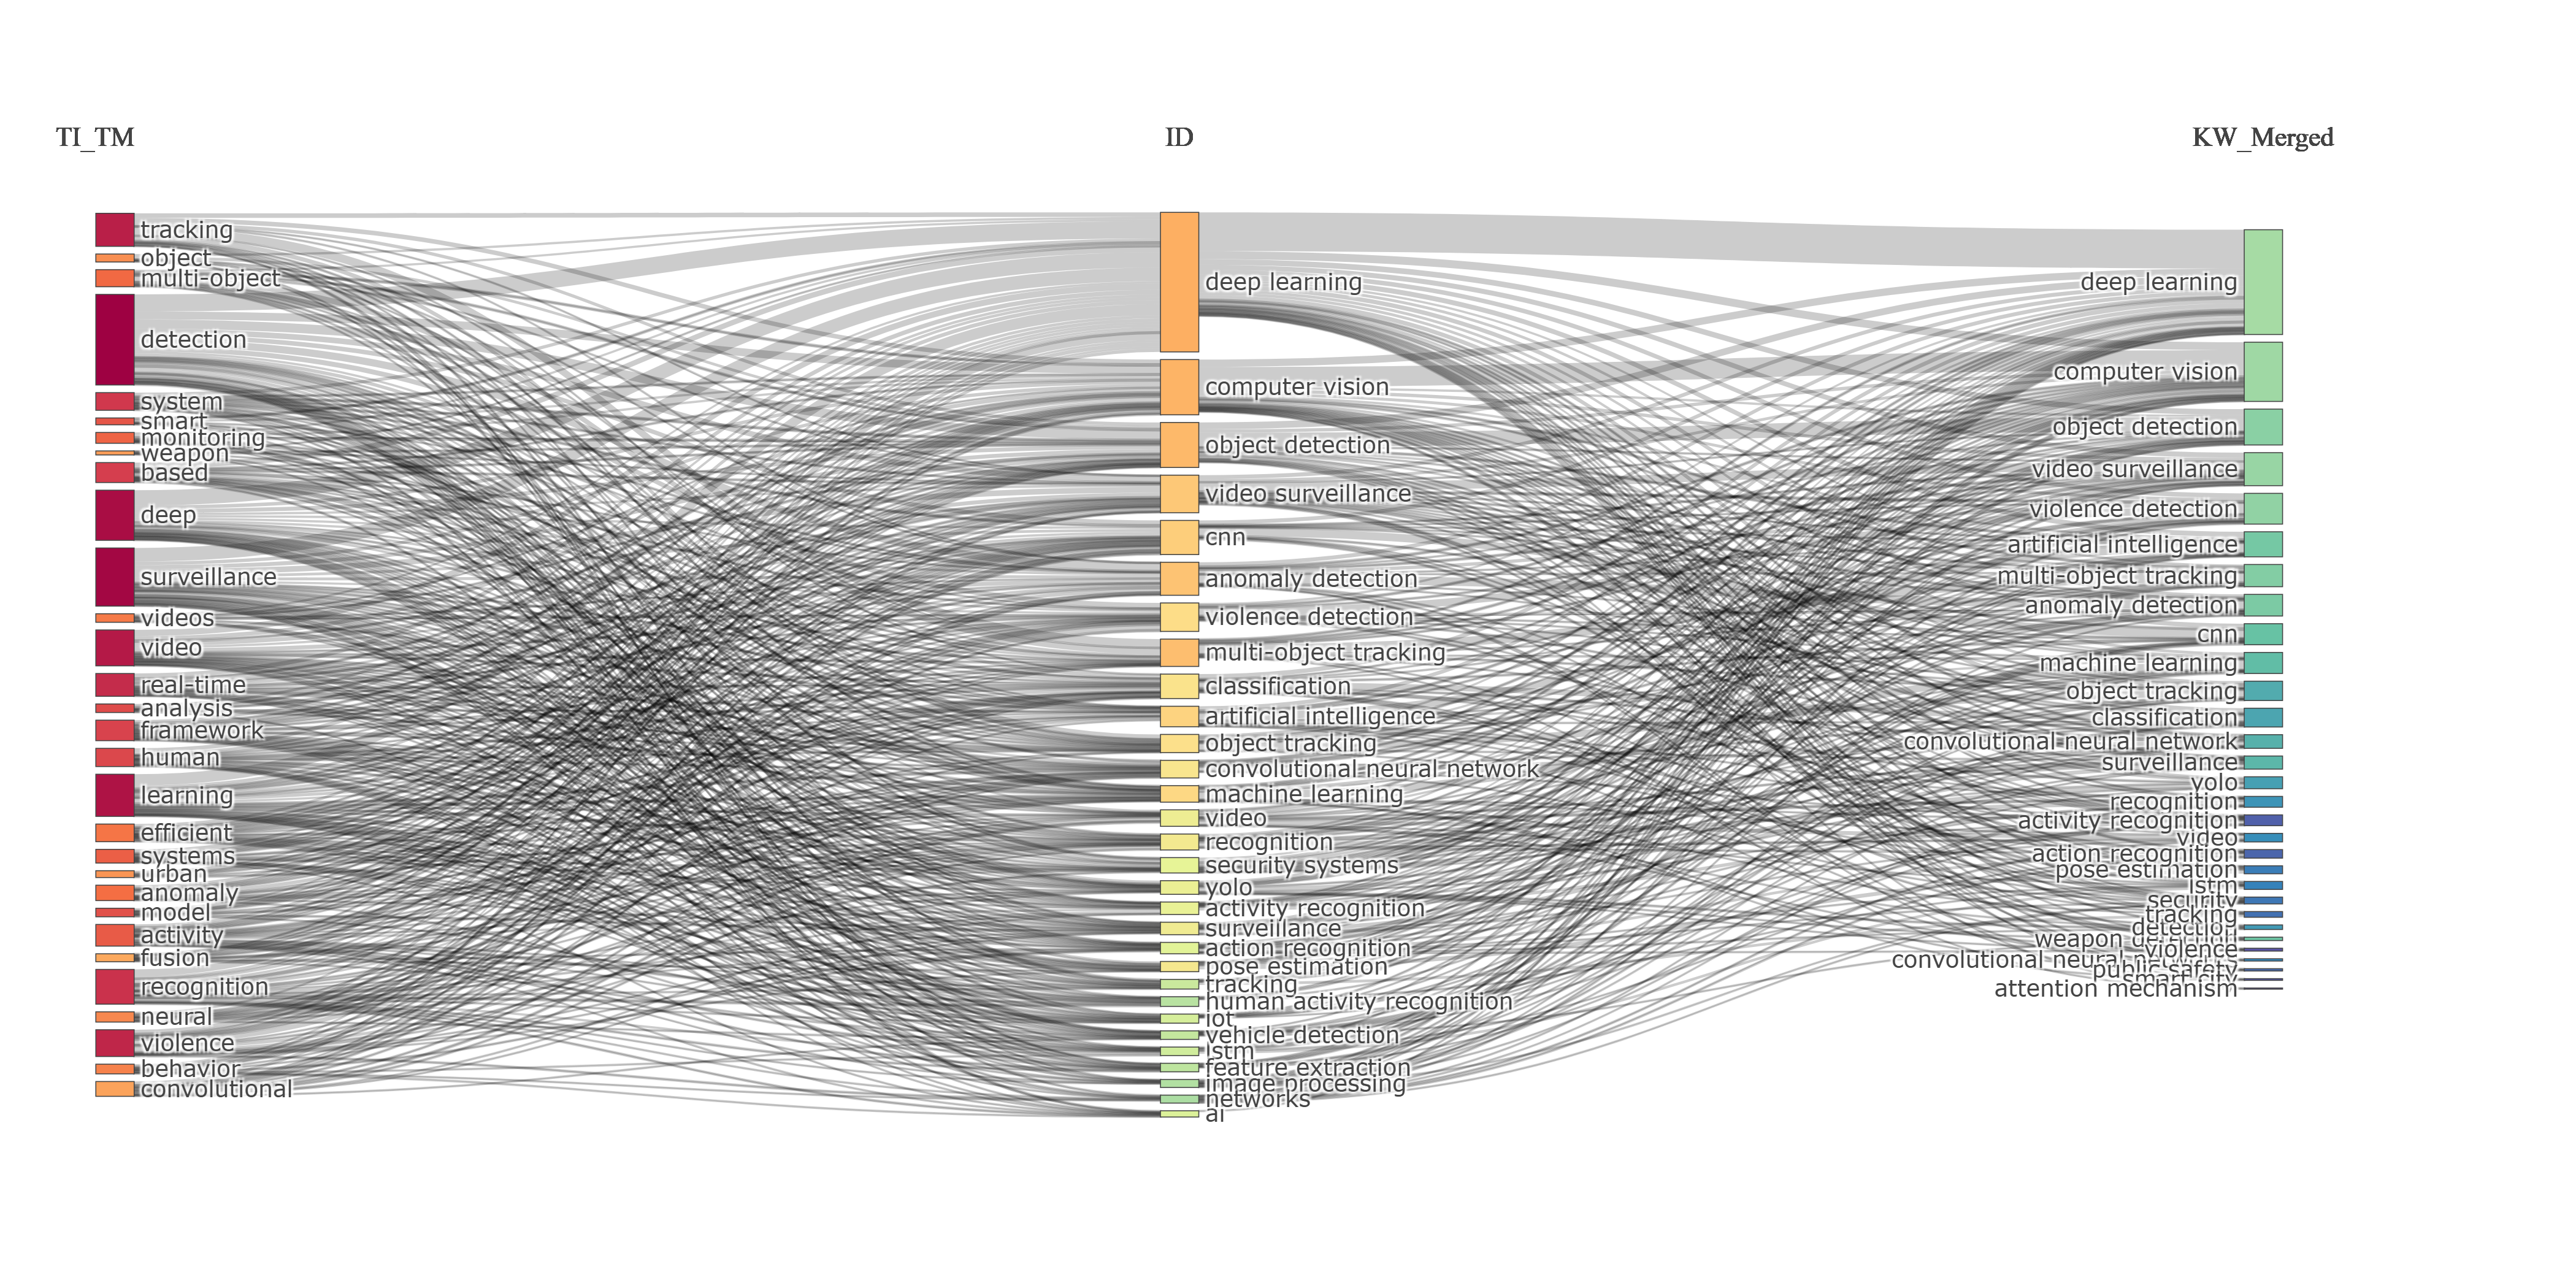
\includegraphics[width=0.98\textwidth]
{ThreeFieldPlot-2026-09-28010254.817106.png}
\caption{Diagrama de tres campos del corpus bibliométrico, que muestra las relaciones
entre los principales componentes bibliográficos analizados.}
\label{fig:threefield}
\end{figure*}


% ------------------------------------------------------------
% AB2
% ------------------------------------------------------------

\subsubsection{AB2: Estructura de la colaboración científica}
\label{subsubsec:ab2}

La producción analizada comprendió afiliaciones procedentes de 50 países.
De los 145 documentos, 45 (31,0\,\%) incluyeron autores afiliados a más de un país,
mientras que 100 (69,0\,\%) correspondieron a publicaciones desarrolladas dentro
de un único país.

La distribución geográfica evidencia una participación importante de países
asiáticos, junto con conexiones con Europa, América y otras regiones. El mapa de
colaboración permite observar los principales vínculos internacionales establecidos
entre los países presentes en el corpus.

\begin{figure*}[htbp]
\centering
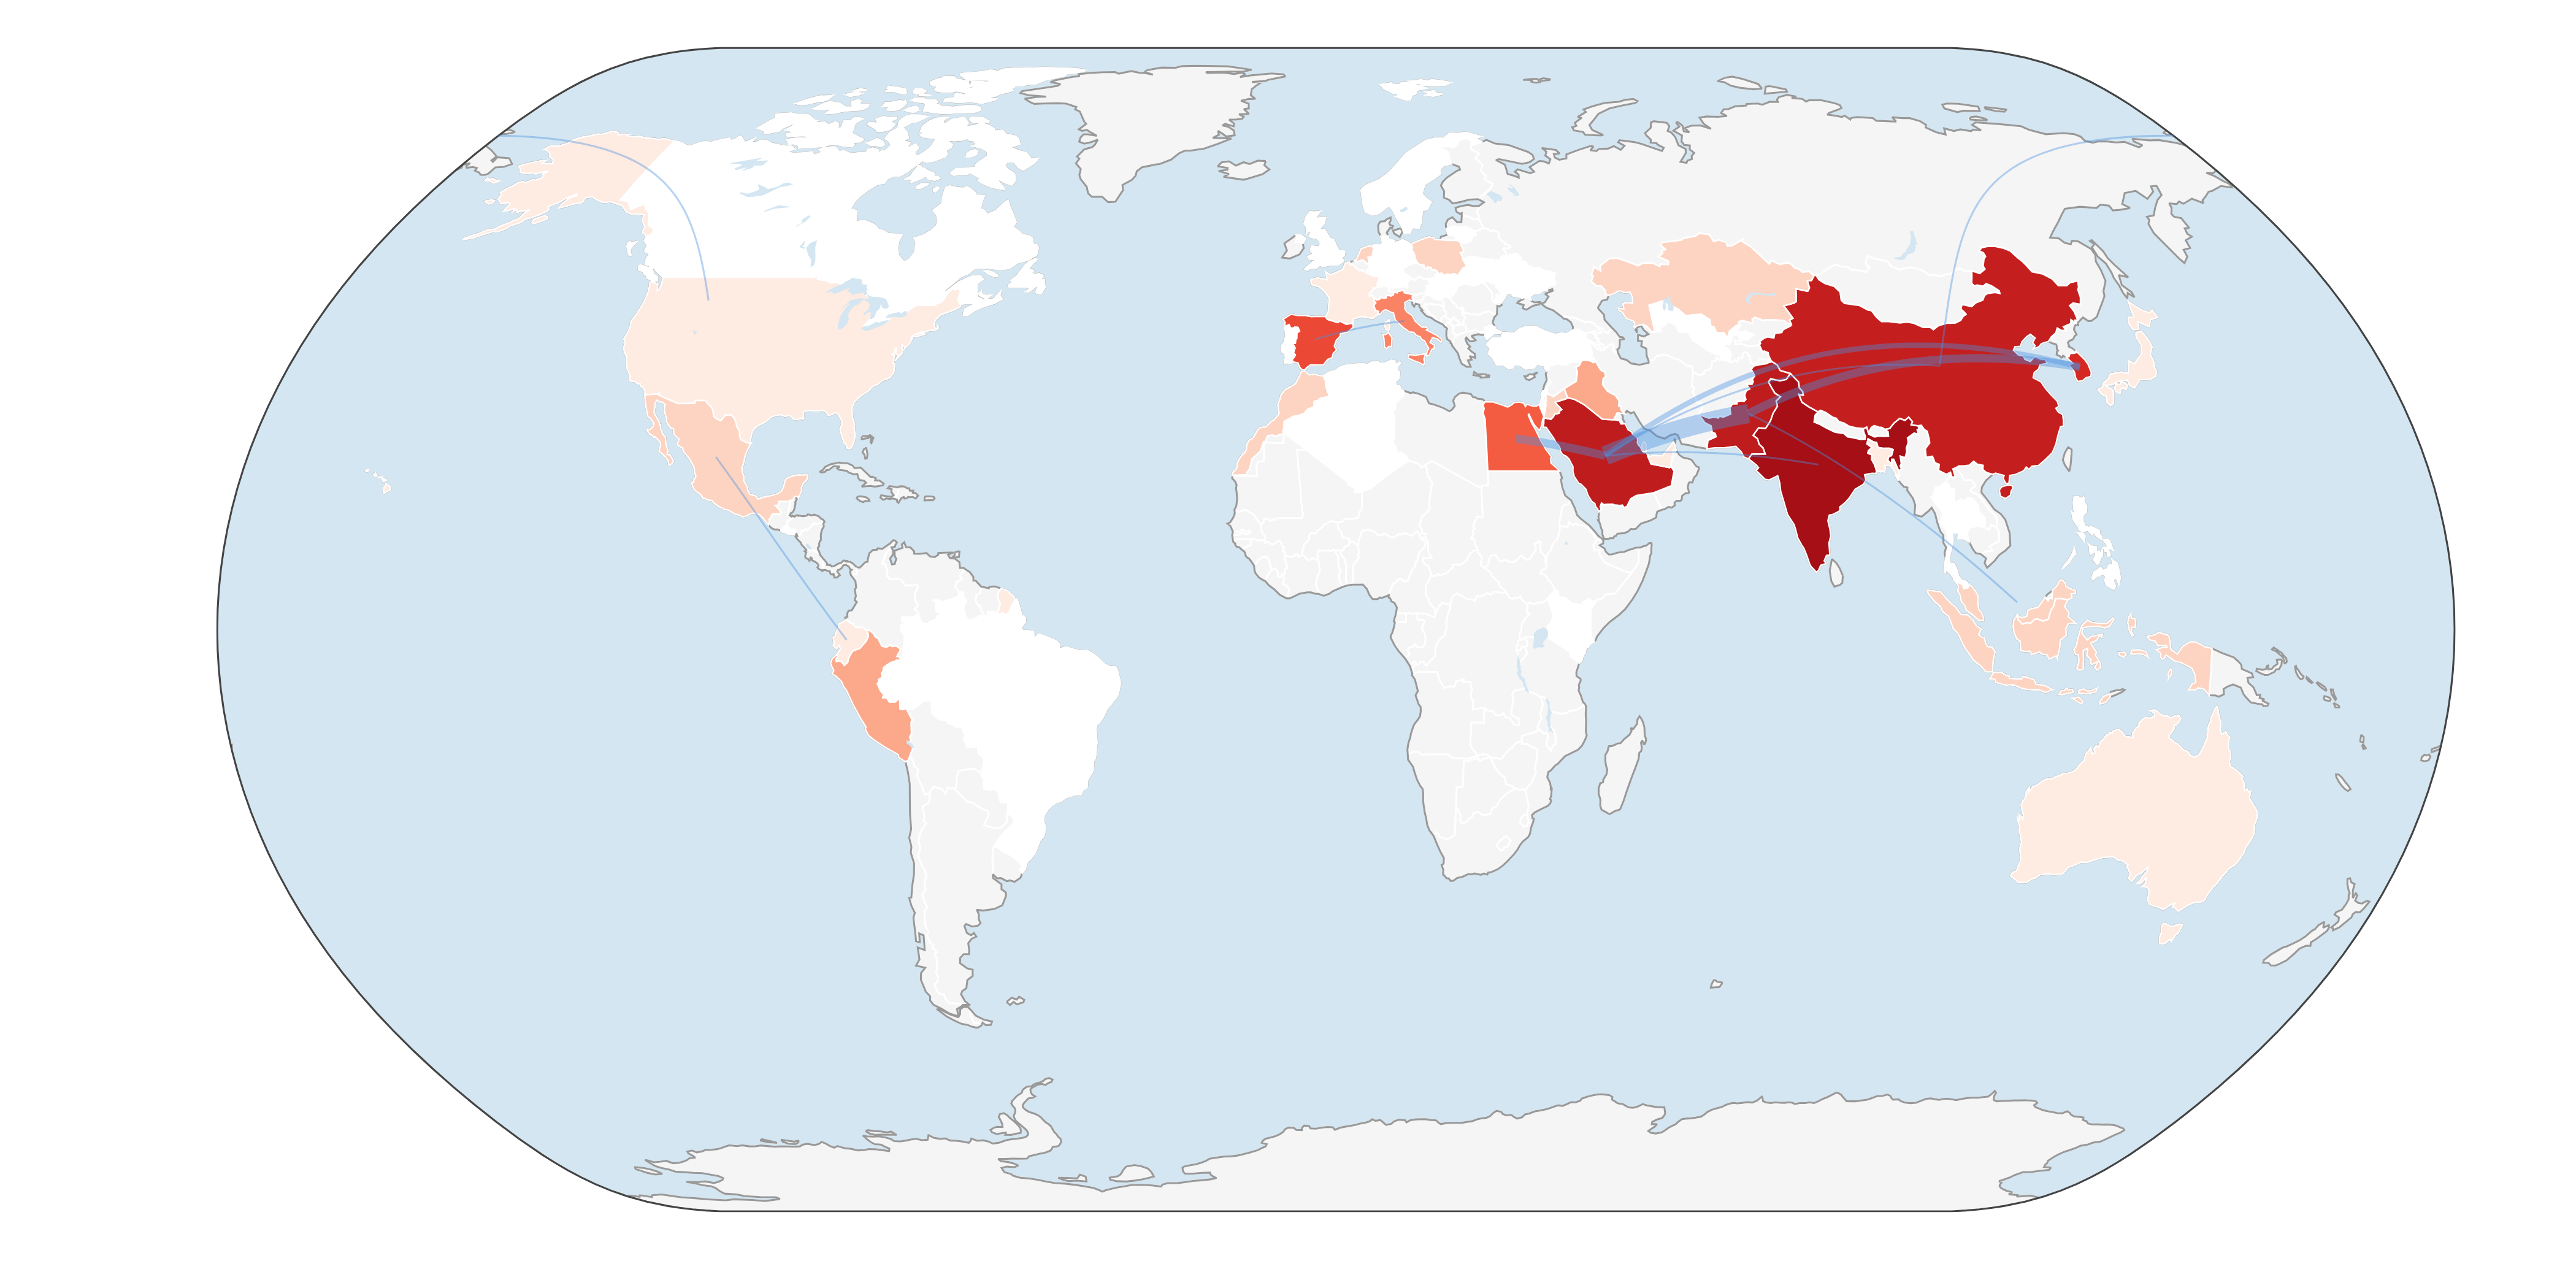
\includegraphics[width=0.96\textwidth]
{CountryCollaborationMap-2026-09-28010452.678578.png}
\caption{Mapa de producción y colaboración científica internacional en el corpus
bibliométrico de Scopus.}
\label{fig:country_collaboration}
\end{figure*}

La red de coautoría muestra, además, la existencia de distintos grupos de
investigadores. Algunos conglomerados presentan conexiones internas densas,
mientras que las relaciones entre grupos son menos frecuentes, lo que sugiere una
estructura constituida por múltiples núcleos de colaboración.

\begin{figure*}[htbp]
\centering
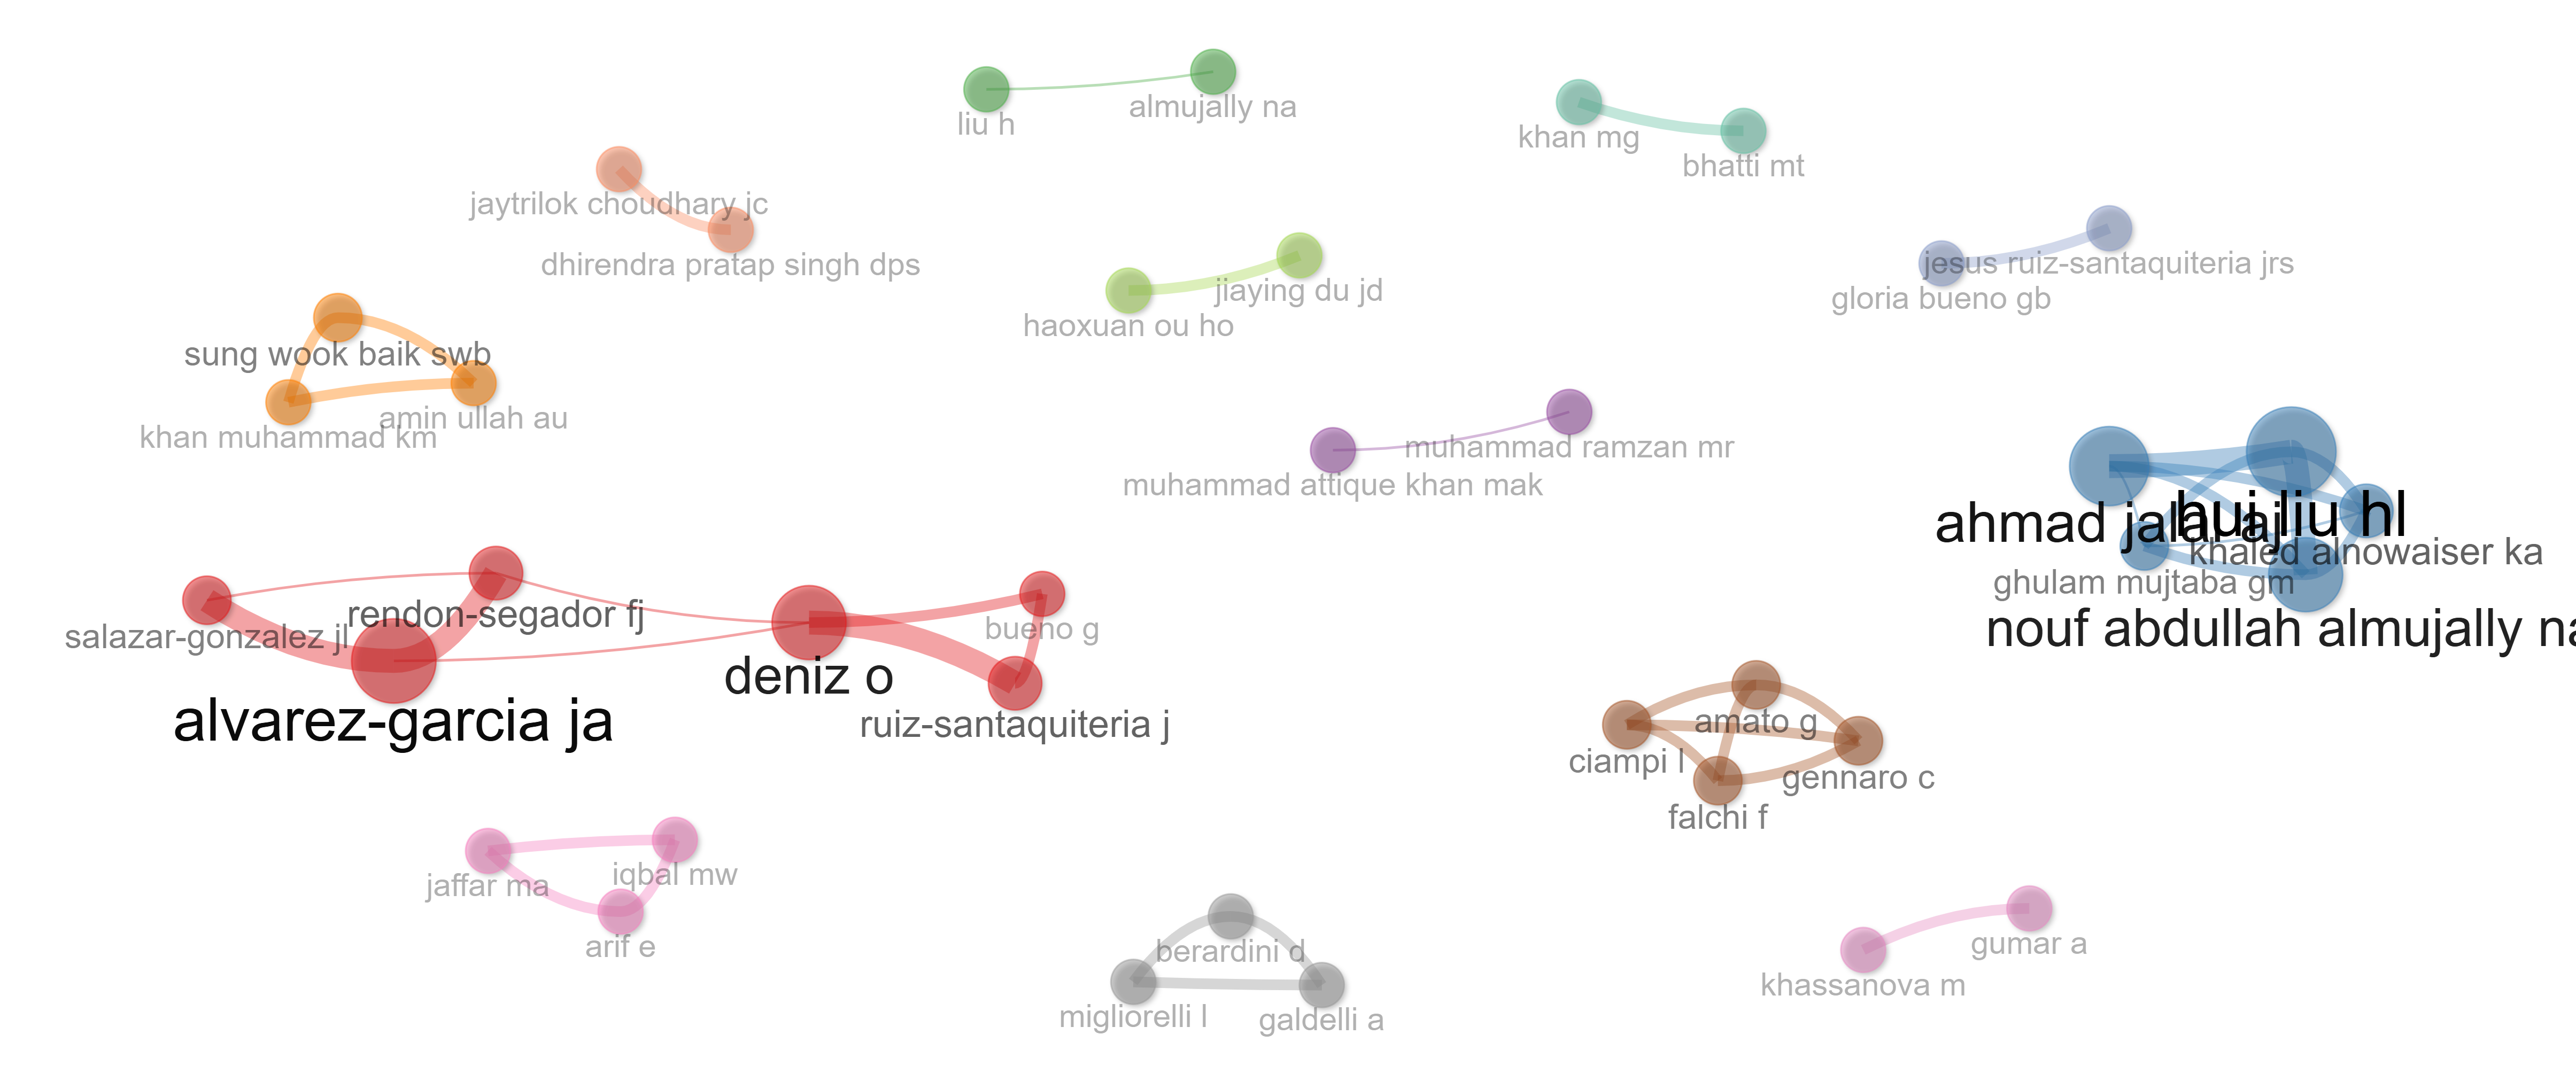
\includegraphics[width=0.96\textwidth]
{Collaboration_Network-2026-09-28010442.151916.png}
\caption{Red de colaboración científica entre autores del corpus bibliométrico.}
\label{fig:collaboration_network}
\end{figure*}


% ------------------------------------------------------------
% AB3
% ------------------------------------------------------------

\subsubsection{AB3: Estructura intelectual y frentes de investigación}
\label{subsubsec:ab3}

La estructura intelectual del campo fue examinada mediante co-citación,
historiografía y acoplamiento bibliográfico. La red de co-citación permite
identificar referencias que son citadas conjuntamente por los documentos del corpus
y, por tanto, forman parte de una base intelectual compartida.

Los agrupamientos identificados muestran diferentes núcleos vinculados con
aprendizaje profundo, detección de violencia, detección de armas, anomalías y
análisis automatizado de video.

\begin{figure*}[htbp]
\centering
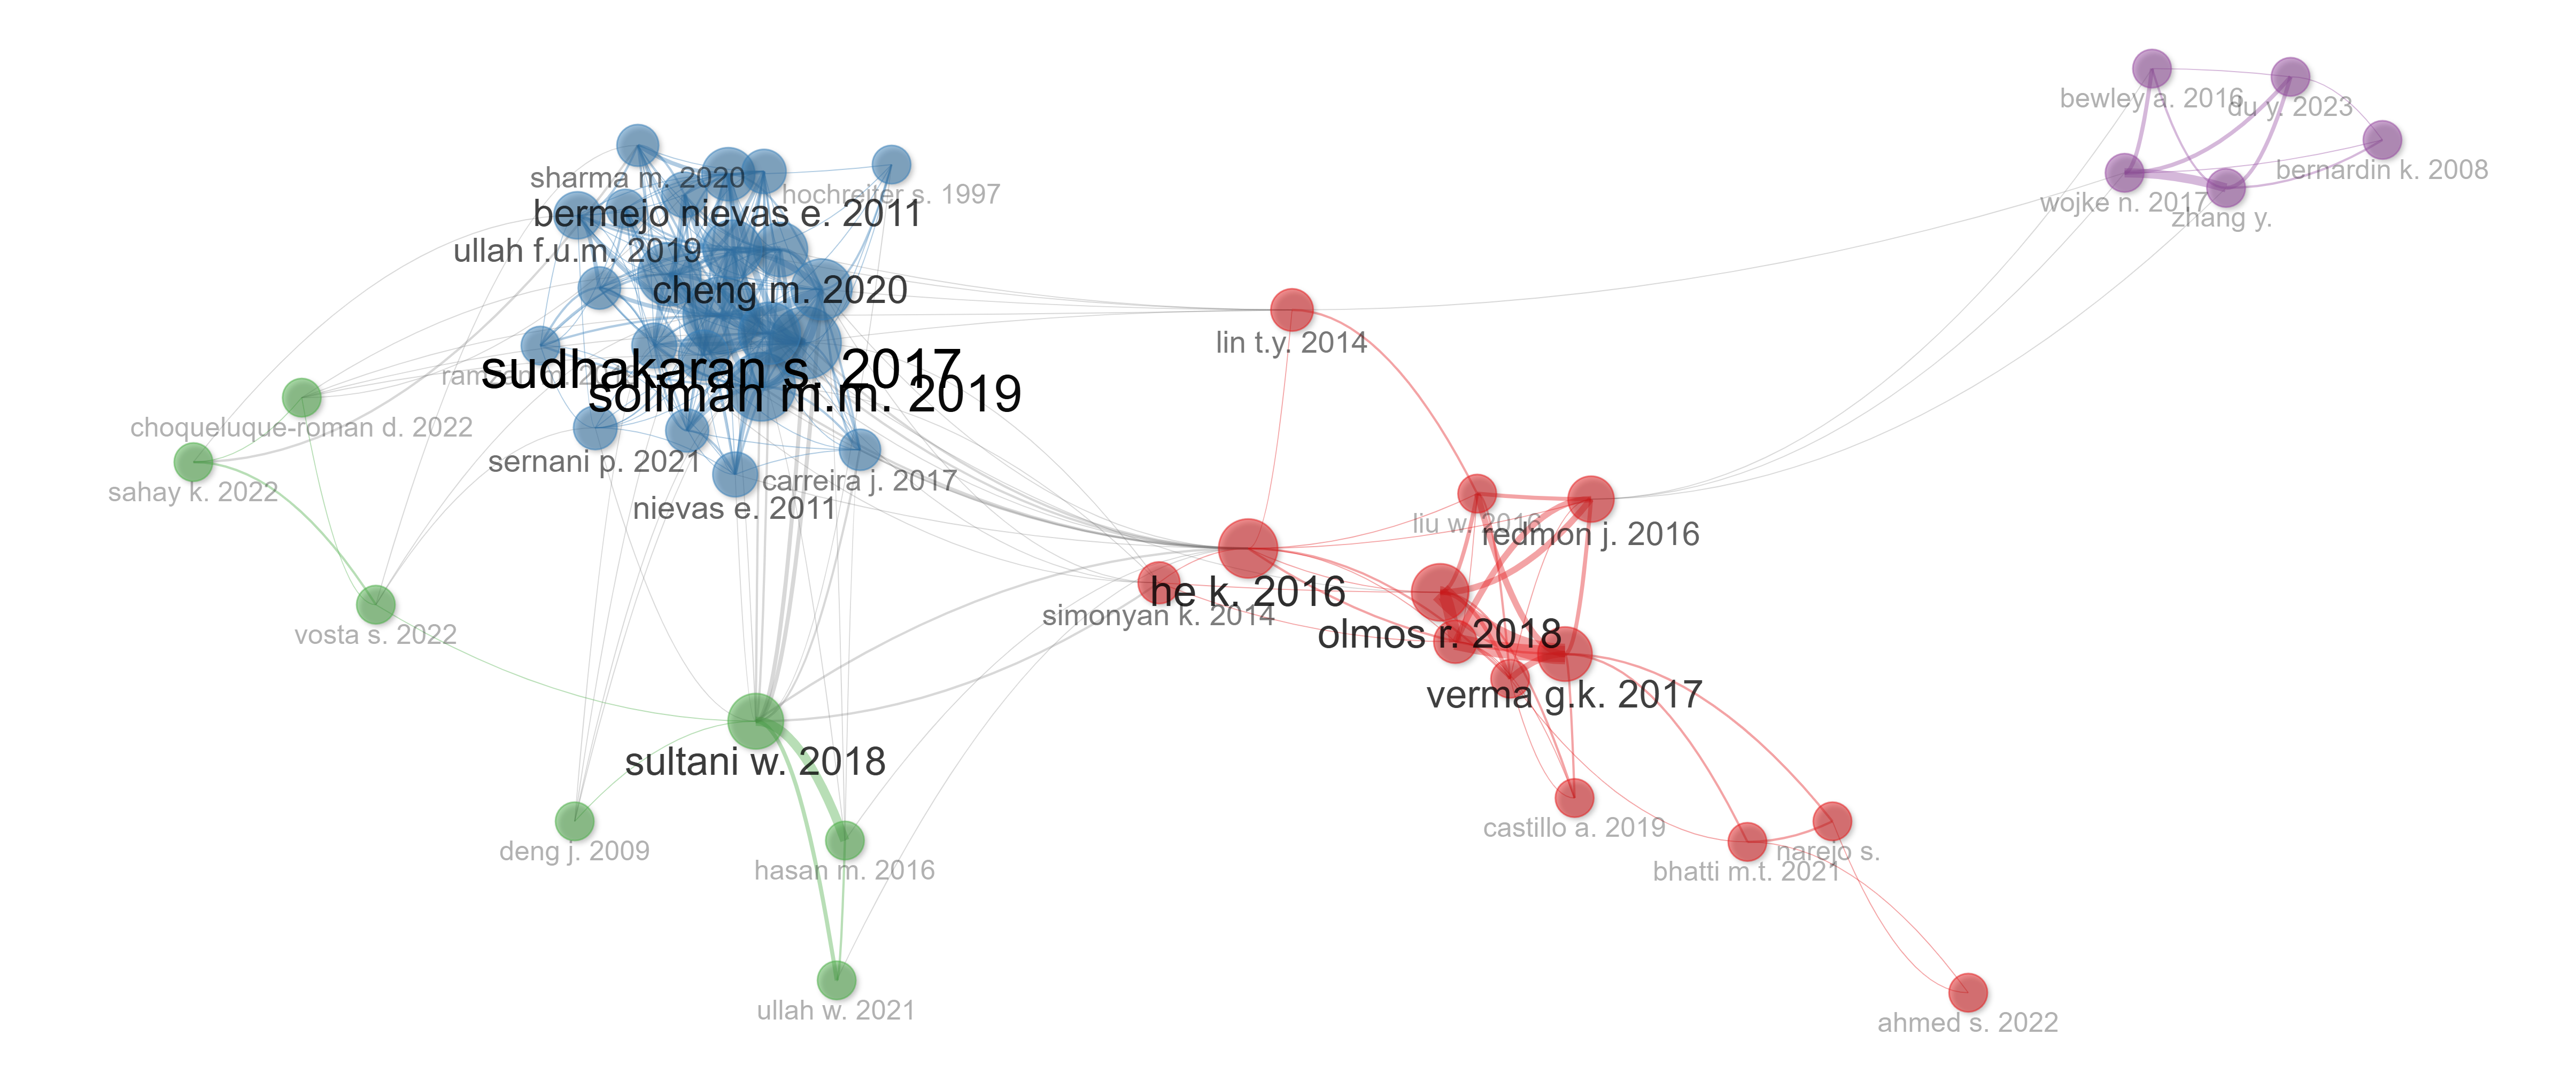
\includegraphics[width=0.97\textwidth]
{Co_citationNetwork-2026-09-29134854.493069.png}
\caption{Red de co-citación del corpus bibliométrico. Los agrupamientos representan
conjuntos de referencias que tienden a ser citadas conjuntamente.}
\label{fig:cocitation_network}
\end{figure*}

El historiograma complementa este análisis representando las relaciones de citación
a través del tiempo. Esta visualización permite reconocer publicaciones que funcionan
como antecedentes de investigaciones posteriores y observar la continuidad de
determinadas líneas de trabajo dentro del periodo estudiado.

\begin{figure*}[htbp]
\centering
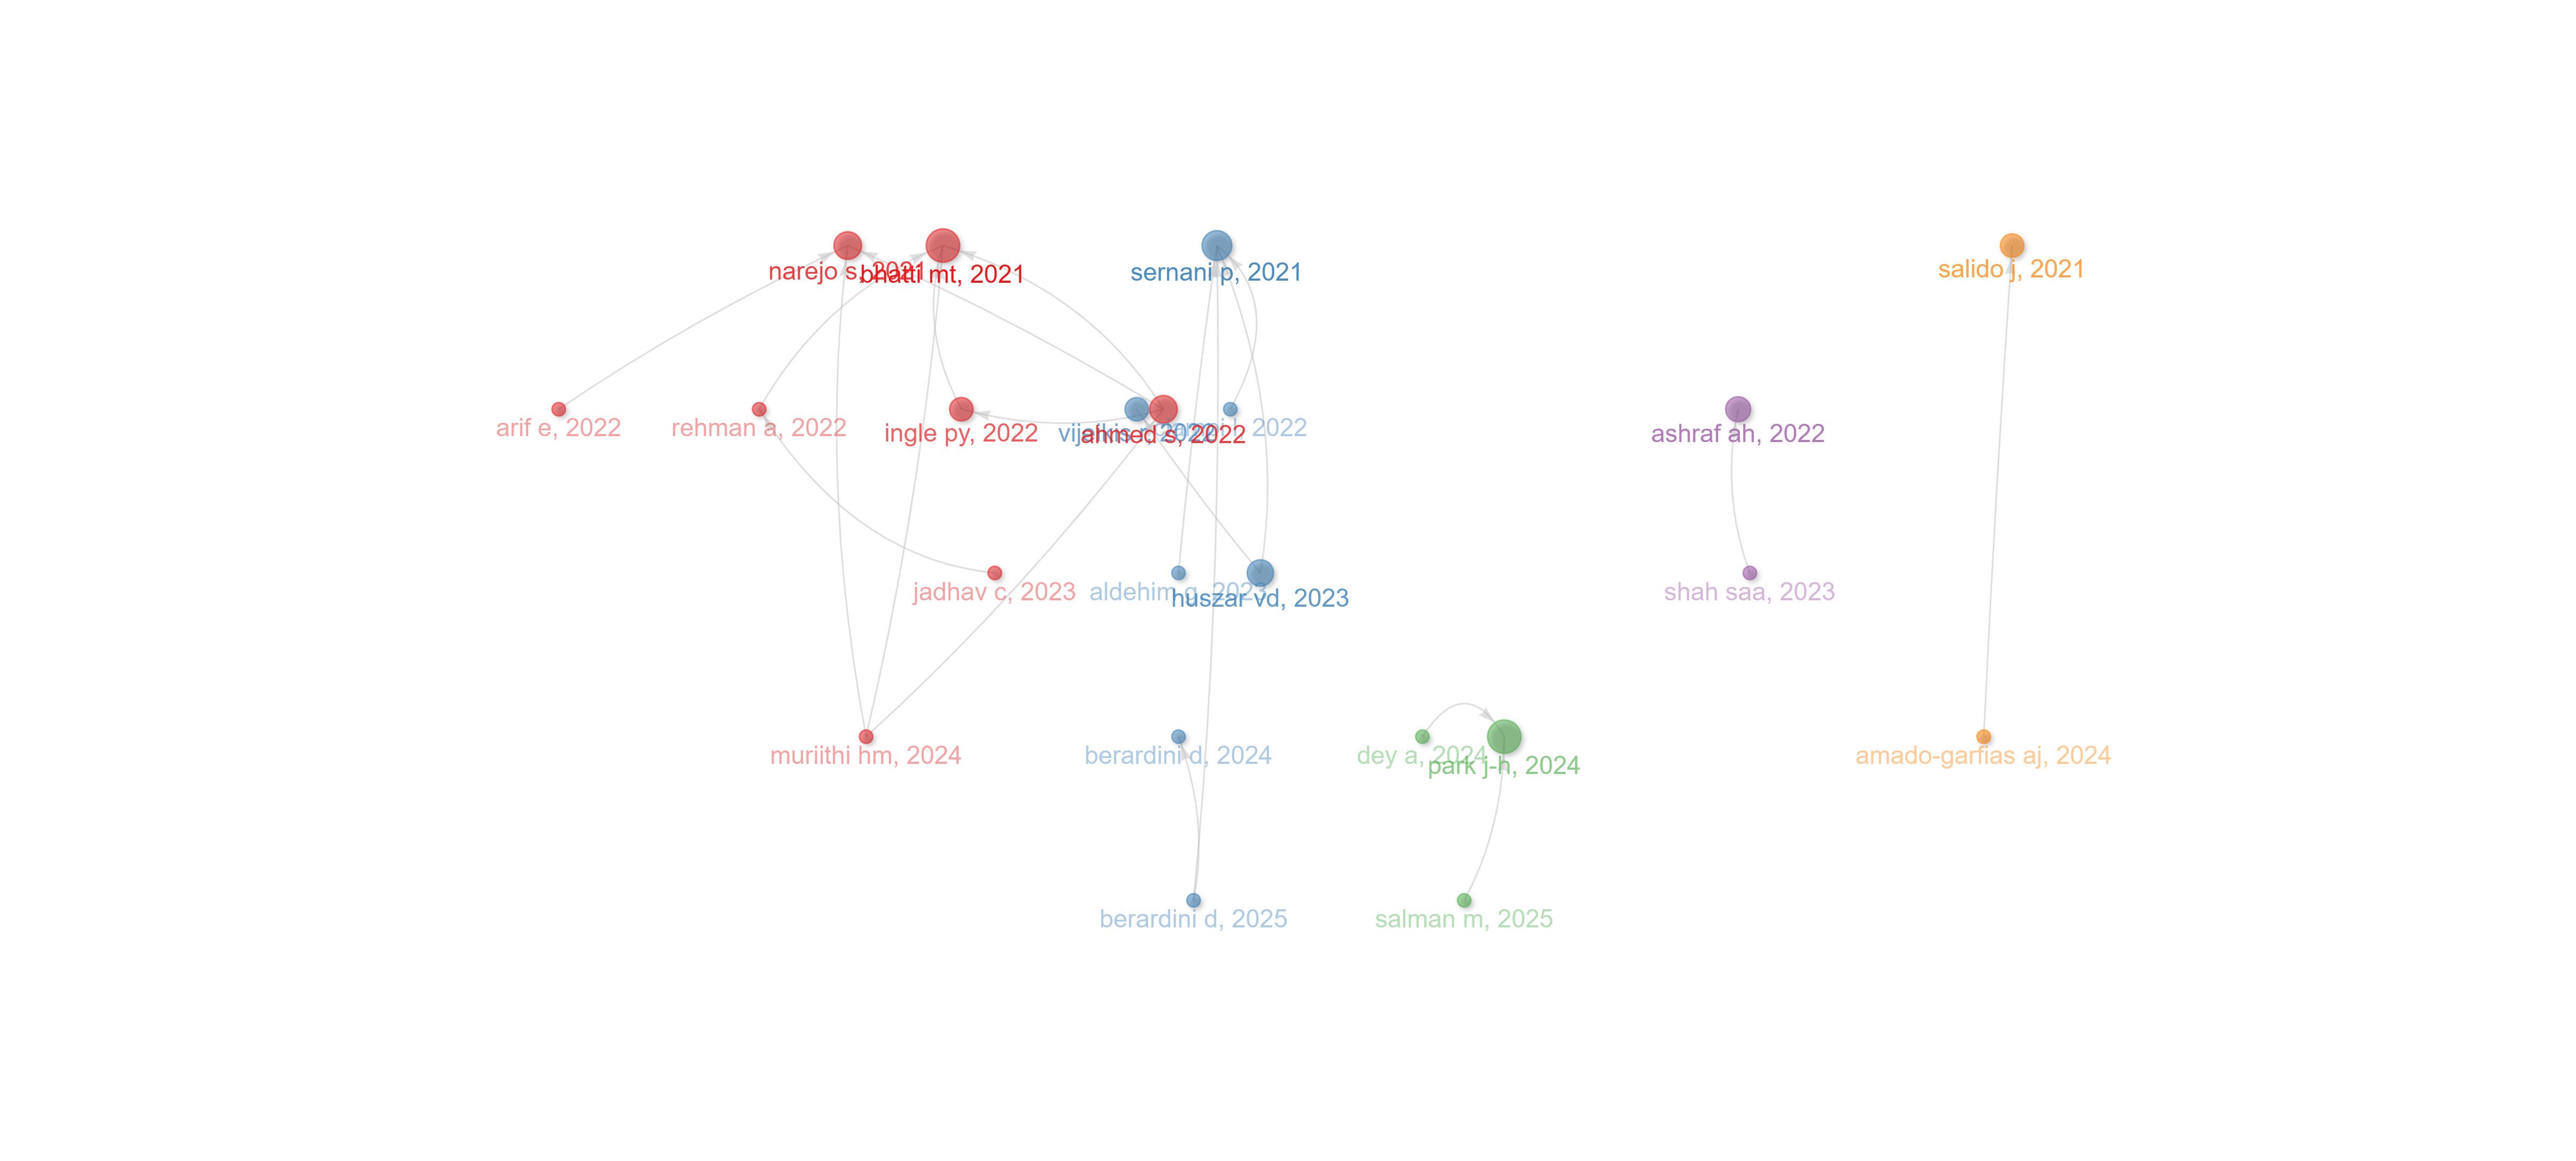
\includegraphics[width=0.97\textwidth]
{Historiograph-2026-09-29134936.207564.png}
\caption{Historiograma de las relaciones de citación entre documentos relevantes
del corpus bibliométrico.}
\label{fig:historiograph}
\end{figure*}

El acoplamiento bibliográfico proporciona una perspectiva complementaria al agrupar
documentos recientes que utilizan referencias similares. Los conglomerados obtenidos
evidencian distintos frentes de investigación relacionados con detección de violencia,
armas, anomalías y seguimiento de objetos.

\begin{figure*}[htbp]
\centering
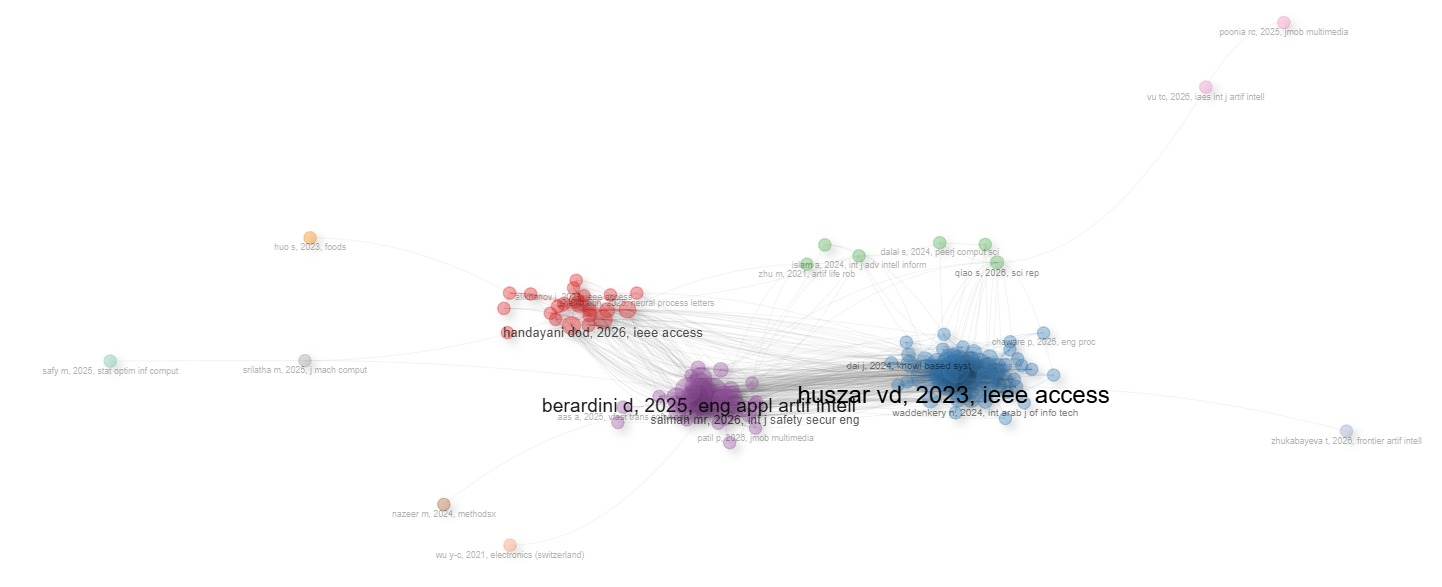
\includegraphics[width=0.97\textwidth]
{Clustering_by_Coupling.png}
\caption{Agrupamiento de documentos mediante acoplamiento bibliográfico. Los nodos
representan publicaciones y los enlaces indican similitud en las referencias utilizadas.}
\label{fig:coupling}
\end{figure*}


% ------------------------------------------------------------
% AB4
% ------------------------------------------------------------

\subsubsection{AB4: Estructura conceptual y evolución temática}
\label{subsubsec:ab4}

Las palabras clave de autor muestran que \textit{deep learning} constituye el término
con mayor presencia, identificado en 67 de los 145 documentos. Le siguen
\textit{video surveillance} (29), \textit{violence detection} (26),
\textit{computer vision} (25), \textit{weapon detection} (22),
\textit{anomaly detection} (13) y \textit{multi-object tracking} (12).

La red de co-ocurrencia muestra que estos conceptos mantienen relaciones frecuentes
entre sí. \textit{Deep learning} ocupa una posición central y se conecta con
videovigilancia, visión por computador, detección de violencia y detección de armas.
En torno a este núcleo aparecen términos más específicos relacionados con anomalías,
seguimiento multiobjeto, reconocimiento de actividades y detección de objetos.

\begin{figure*}[htbp]
\centering
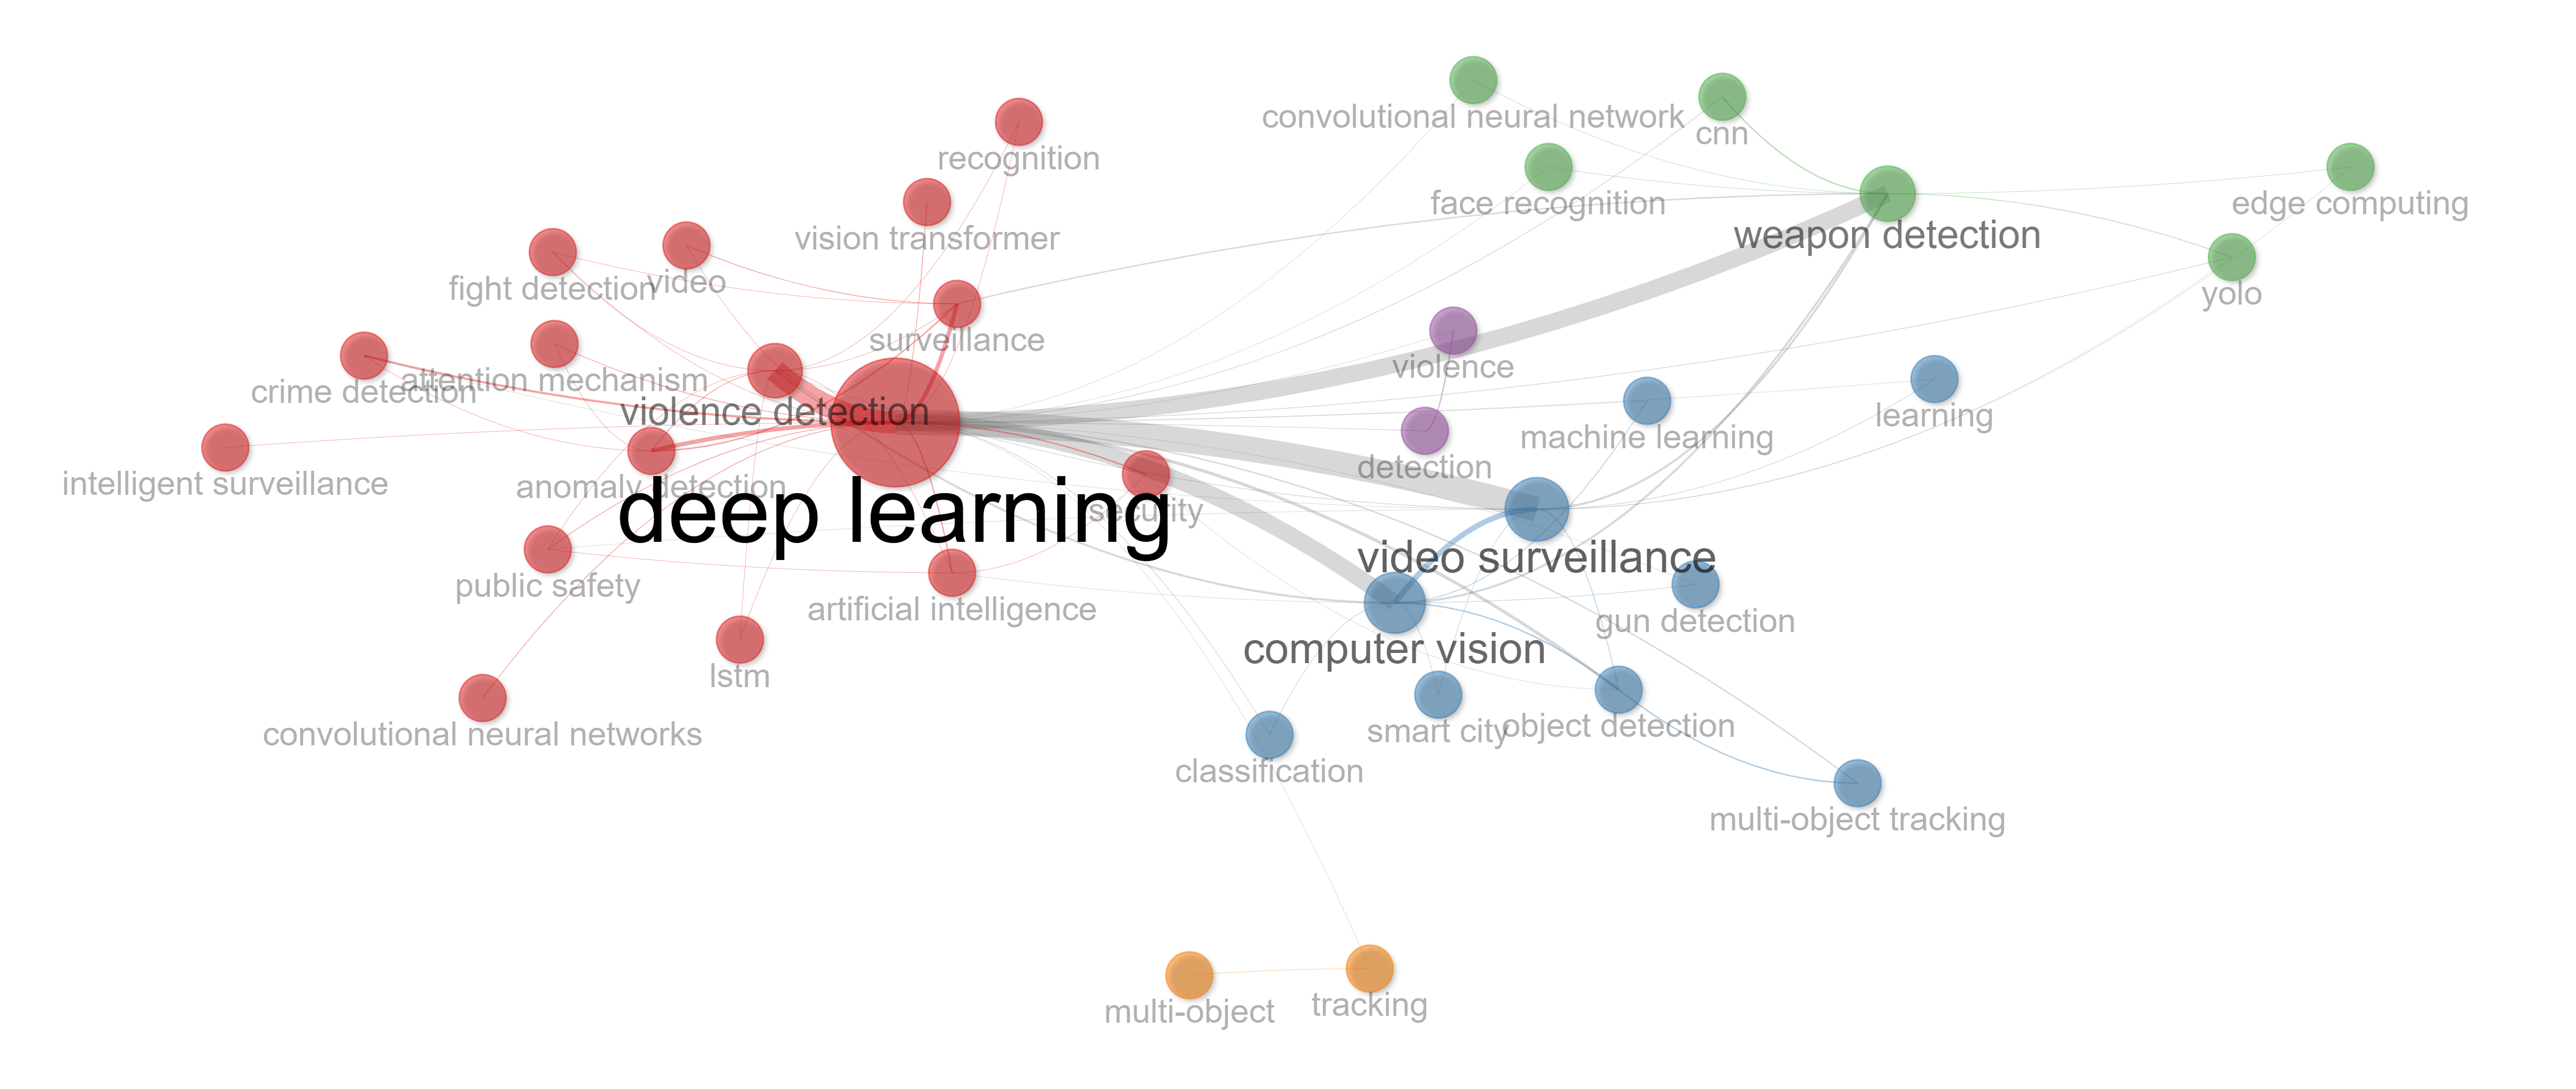
\includegraphics[width=0.97\textwidth]
{Co_occurrenceNetwork-2026-10-04220412.241765.png}
\caption{Red de co-ocurrencia de palabras clave del corpus bibliométrico.}
\label{fig:cooccurrence}
\end{figure*}

La distribución temporal permite identificar cambios en el énfasis temático.
Durante 2021--2022 predominaron \textit{deep learning}, videovigilancia,
visión por computador, detección de violencia y detección de armas.
En 2023--2024 se mantuvieron estos núcleos y aumentó la presencia de términos
asociados con vigilancia inteligente, ciudades inteligentes y seguimiento
multiobjeto. Durante 2025--2026 se incrementó la frecuencia relativa de
\textit{weapon detection}, \textit{anomaly detection},
\textit{multi-object tracking}, YOLO y mecanismos de atención.

\begin{table*}[htbp]
\caption{Evolución de las principales palabras clave de autor por periodo}
\label{tab:ab4_keywords}
\centering
\small
\renewcommand{\arraystretch}{1.12}
\begin{tabular}{@{}L{2.6cm}L{9.8cm}@{}}
\toprule
\textbf{Periodo} & \textbf{Términos con mayor presencia} \\
\midrule

2021--2022 &
Deep learning (12), video surveillance (8), computer vision (7),
violence detection (7), weapon detection (5), object detection (4) \\

2023--2024 &
Deep learning (24), computer vision (11), video surveillance (10),
violence detection (9), weapon detection (5), multi-object tracking (3),
smart surveillance (3) \\

2025--2026 &
Deep learning (31), weapon detection (12), video surveillance (11),
violence detection (10), anomaly detection (8), multi-object tracking (7),
YOLO (5), attention mechanism (4) \\

\bottomrule
\end{tabular}
\end{table*}

El mapa temático permite representar los temas identificados según su desarrollo
y su relación con el resto del campo, diferenciando núcleos centrales de líneas
más específicas o emergentes.

\begin{figure*}[htbp]
\centering
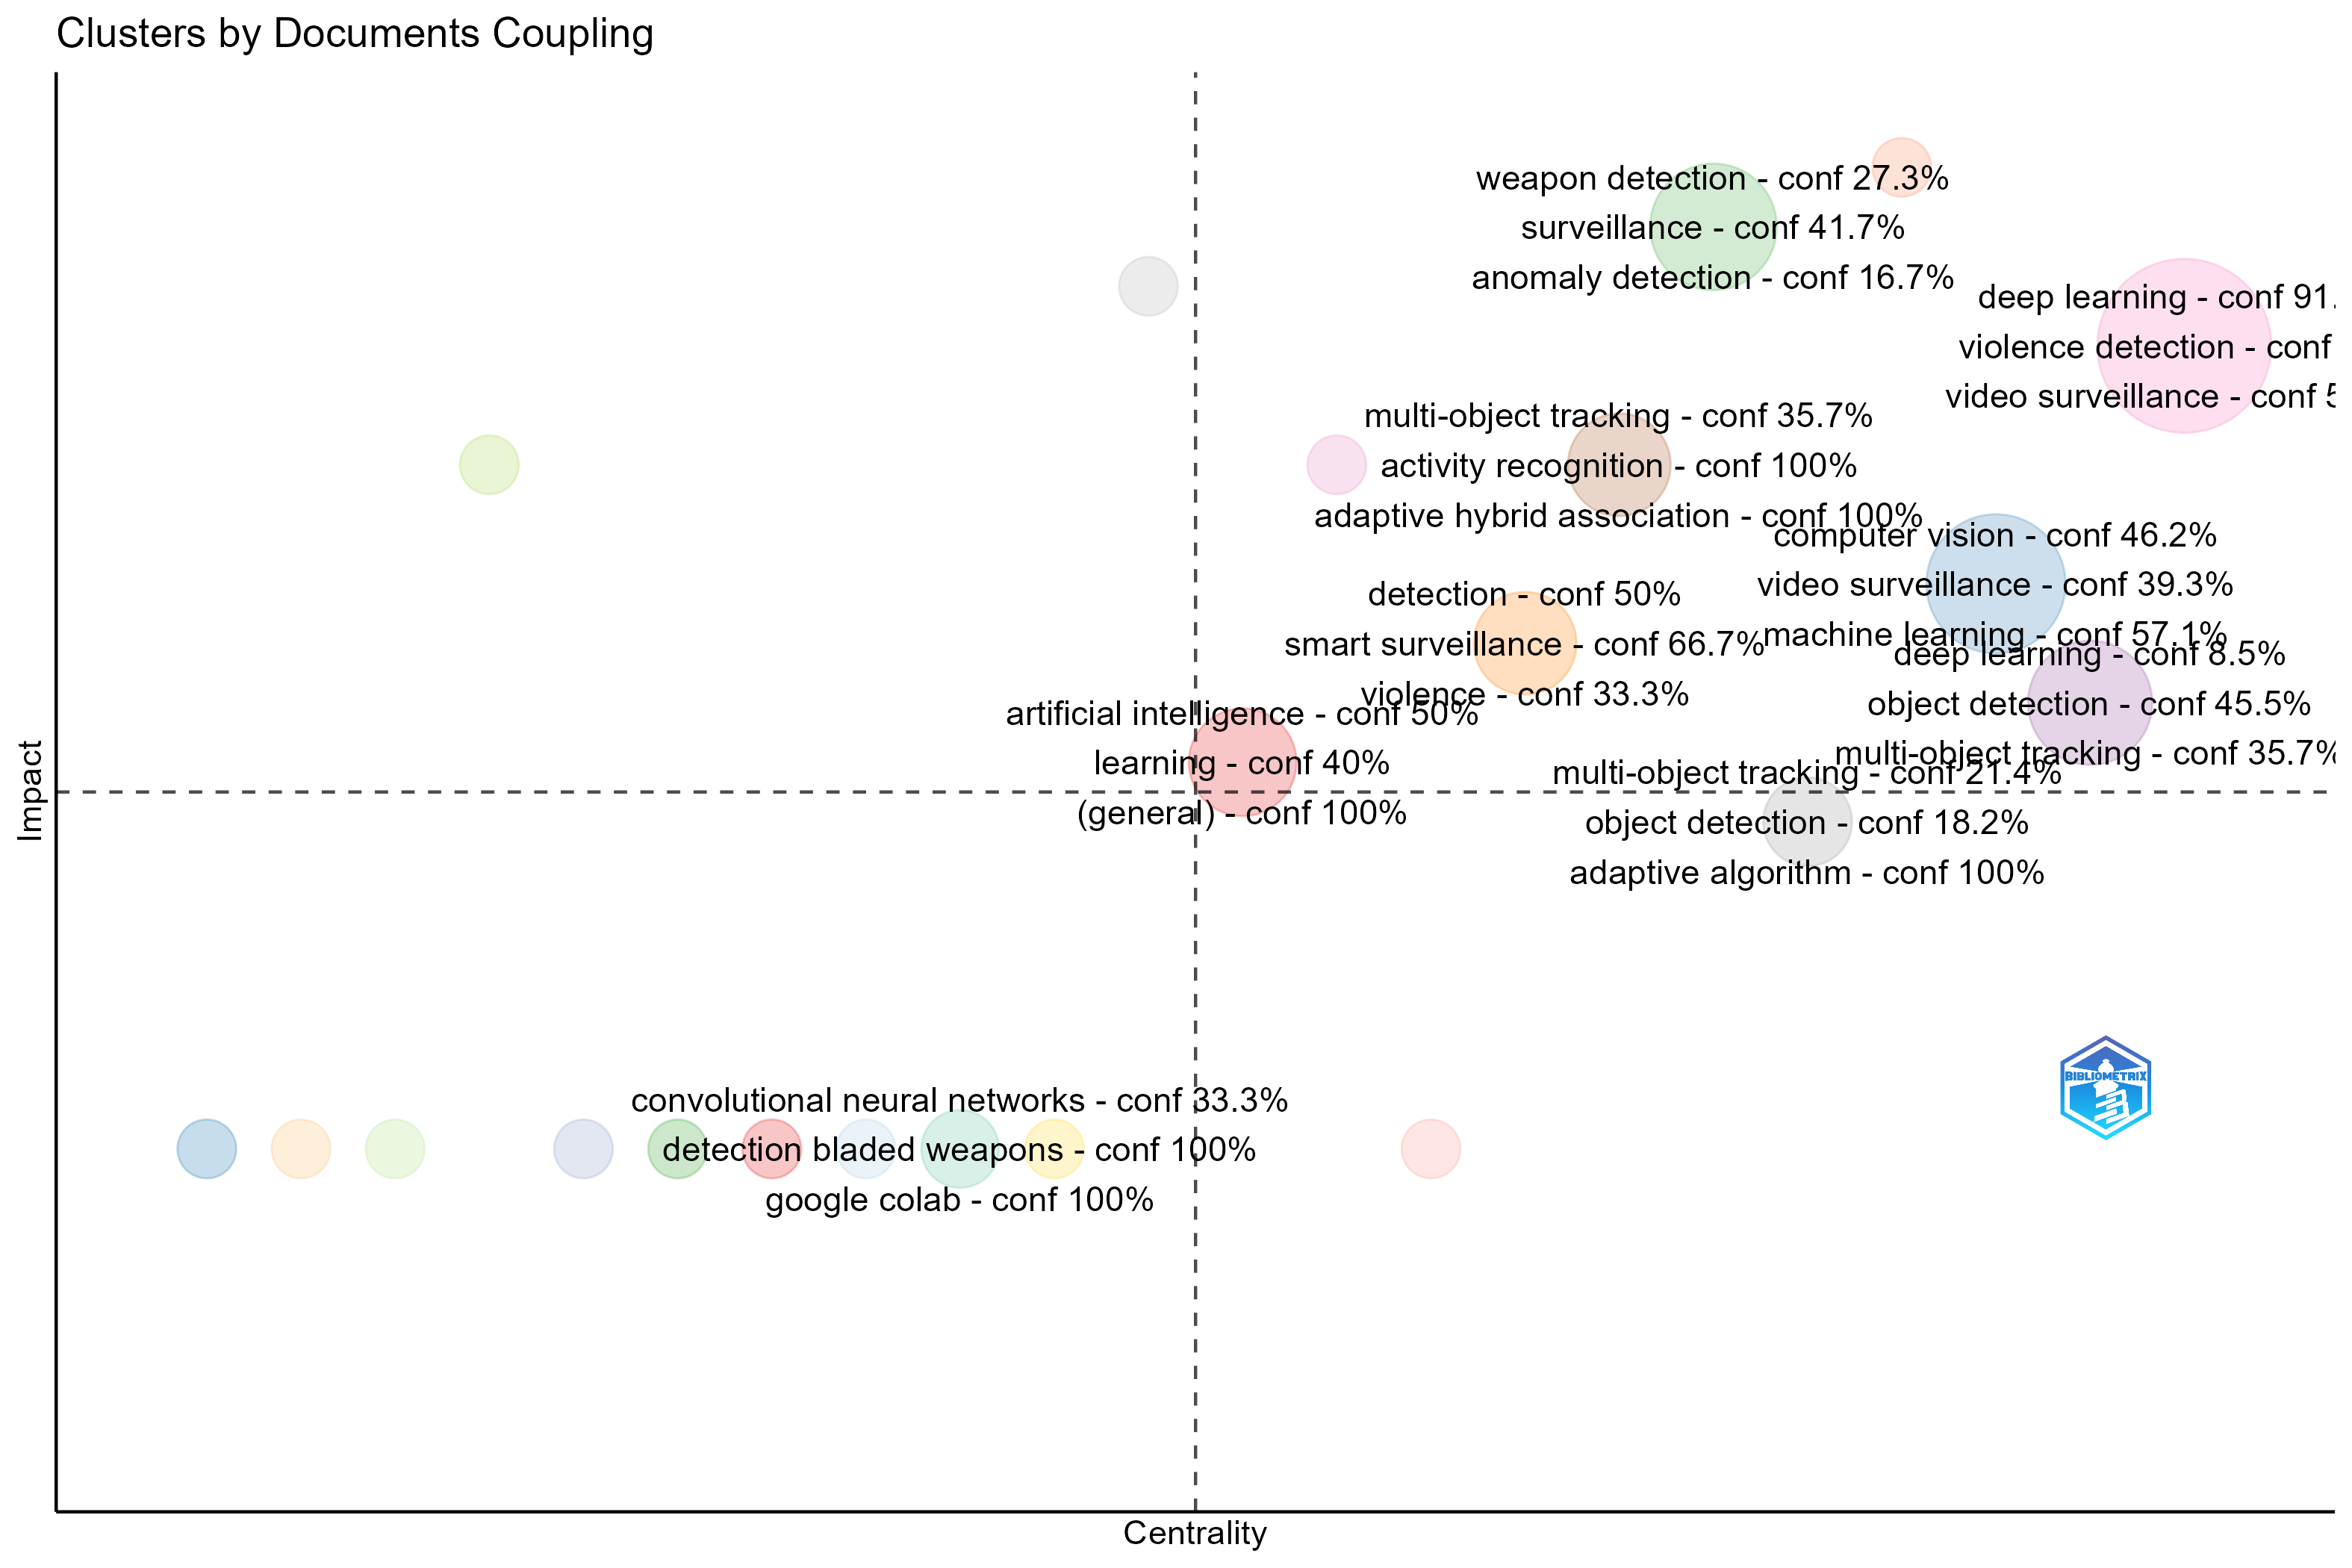
\includegraphics[width=0.92\textwidth]
{CouplingMap-2026-09-28 (1).png}
\caption{Mapa temático obtenido mediante análisis de acoplamiento bibliográfico.}
\label{fig:thematic_map}
\end{figure*}

El análisis factorial proporciona una representación adicional de la estructura
conceptual, permitiendo observar la proximidad entre términos que presentan patrones
similares de aparición dentro del corpus.

\begin{figure*}[htbp]
\centering
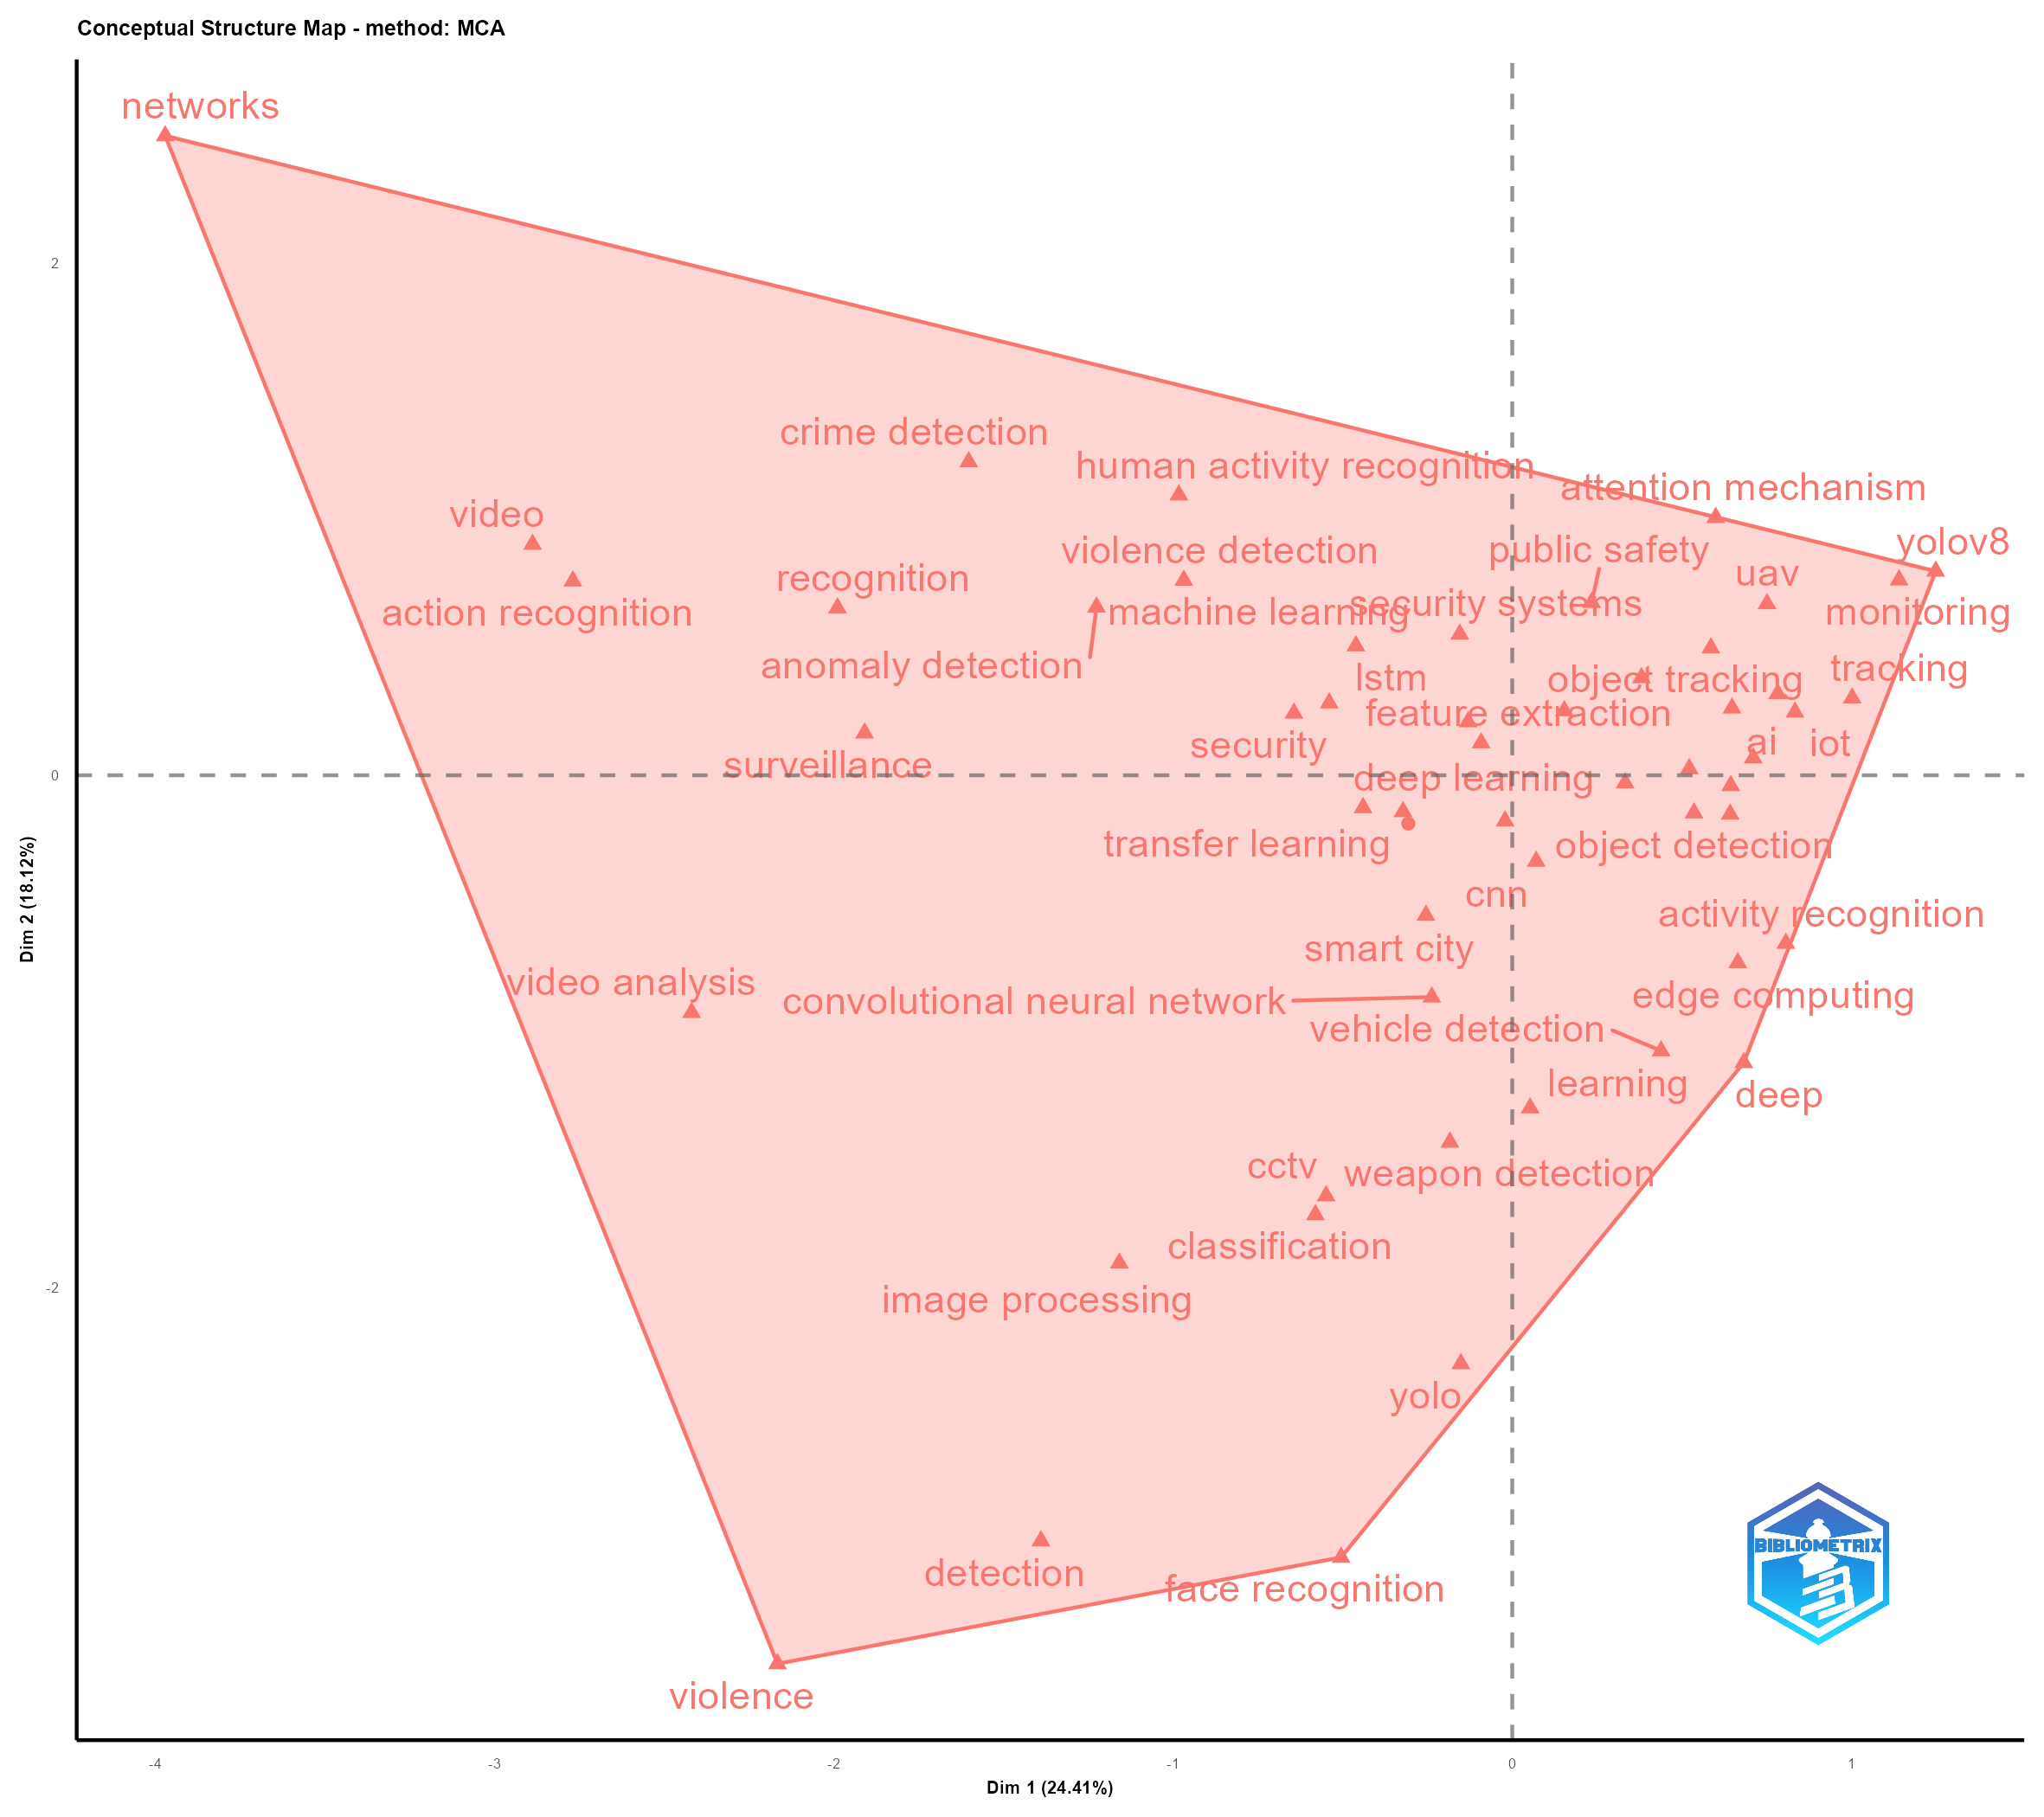
\includegraphics[width=0.90\textwidth]
{FactorialMap_2026-09-28.png}
\caption{Mapa factorial de la estructura conceptual del corpus bibliométrico.}
\label{fig:factorial_map}
\end{figure*}

Finalmente, la nube de palabras presenta de manera visual la frecuencia relativa
de los conceptos empleados en las publicaciones y permite reconocer rápidamente
los términos con mayor presencia dentro del corpus.

\begin{figure}[htbp]
\centering
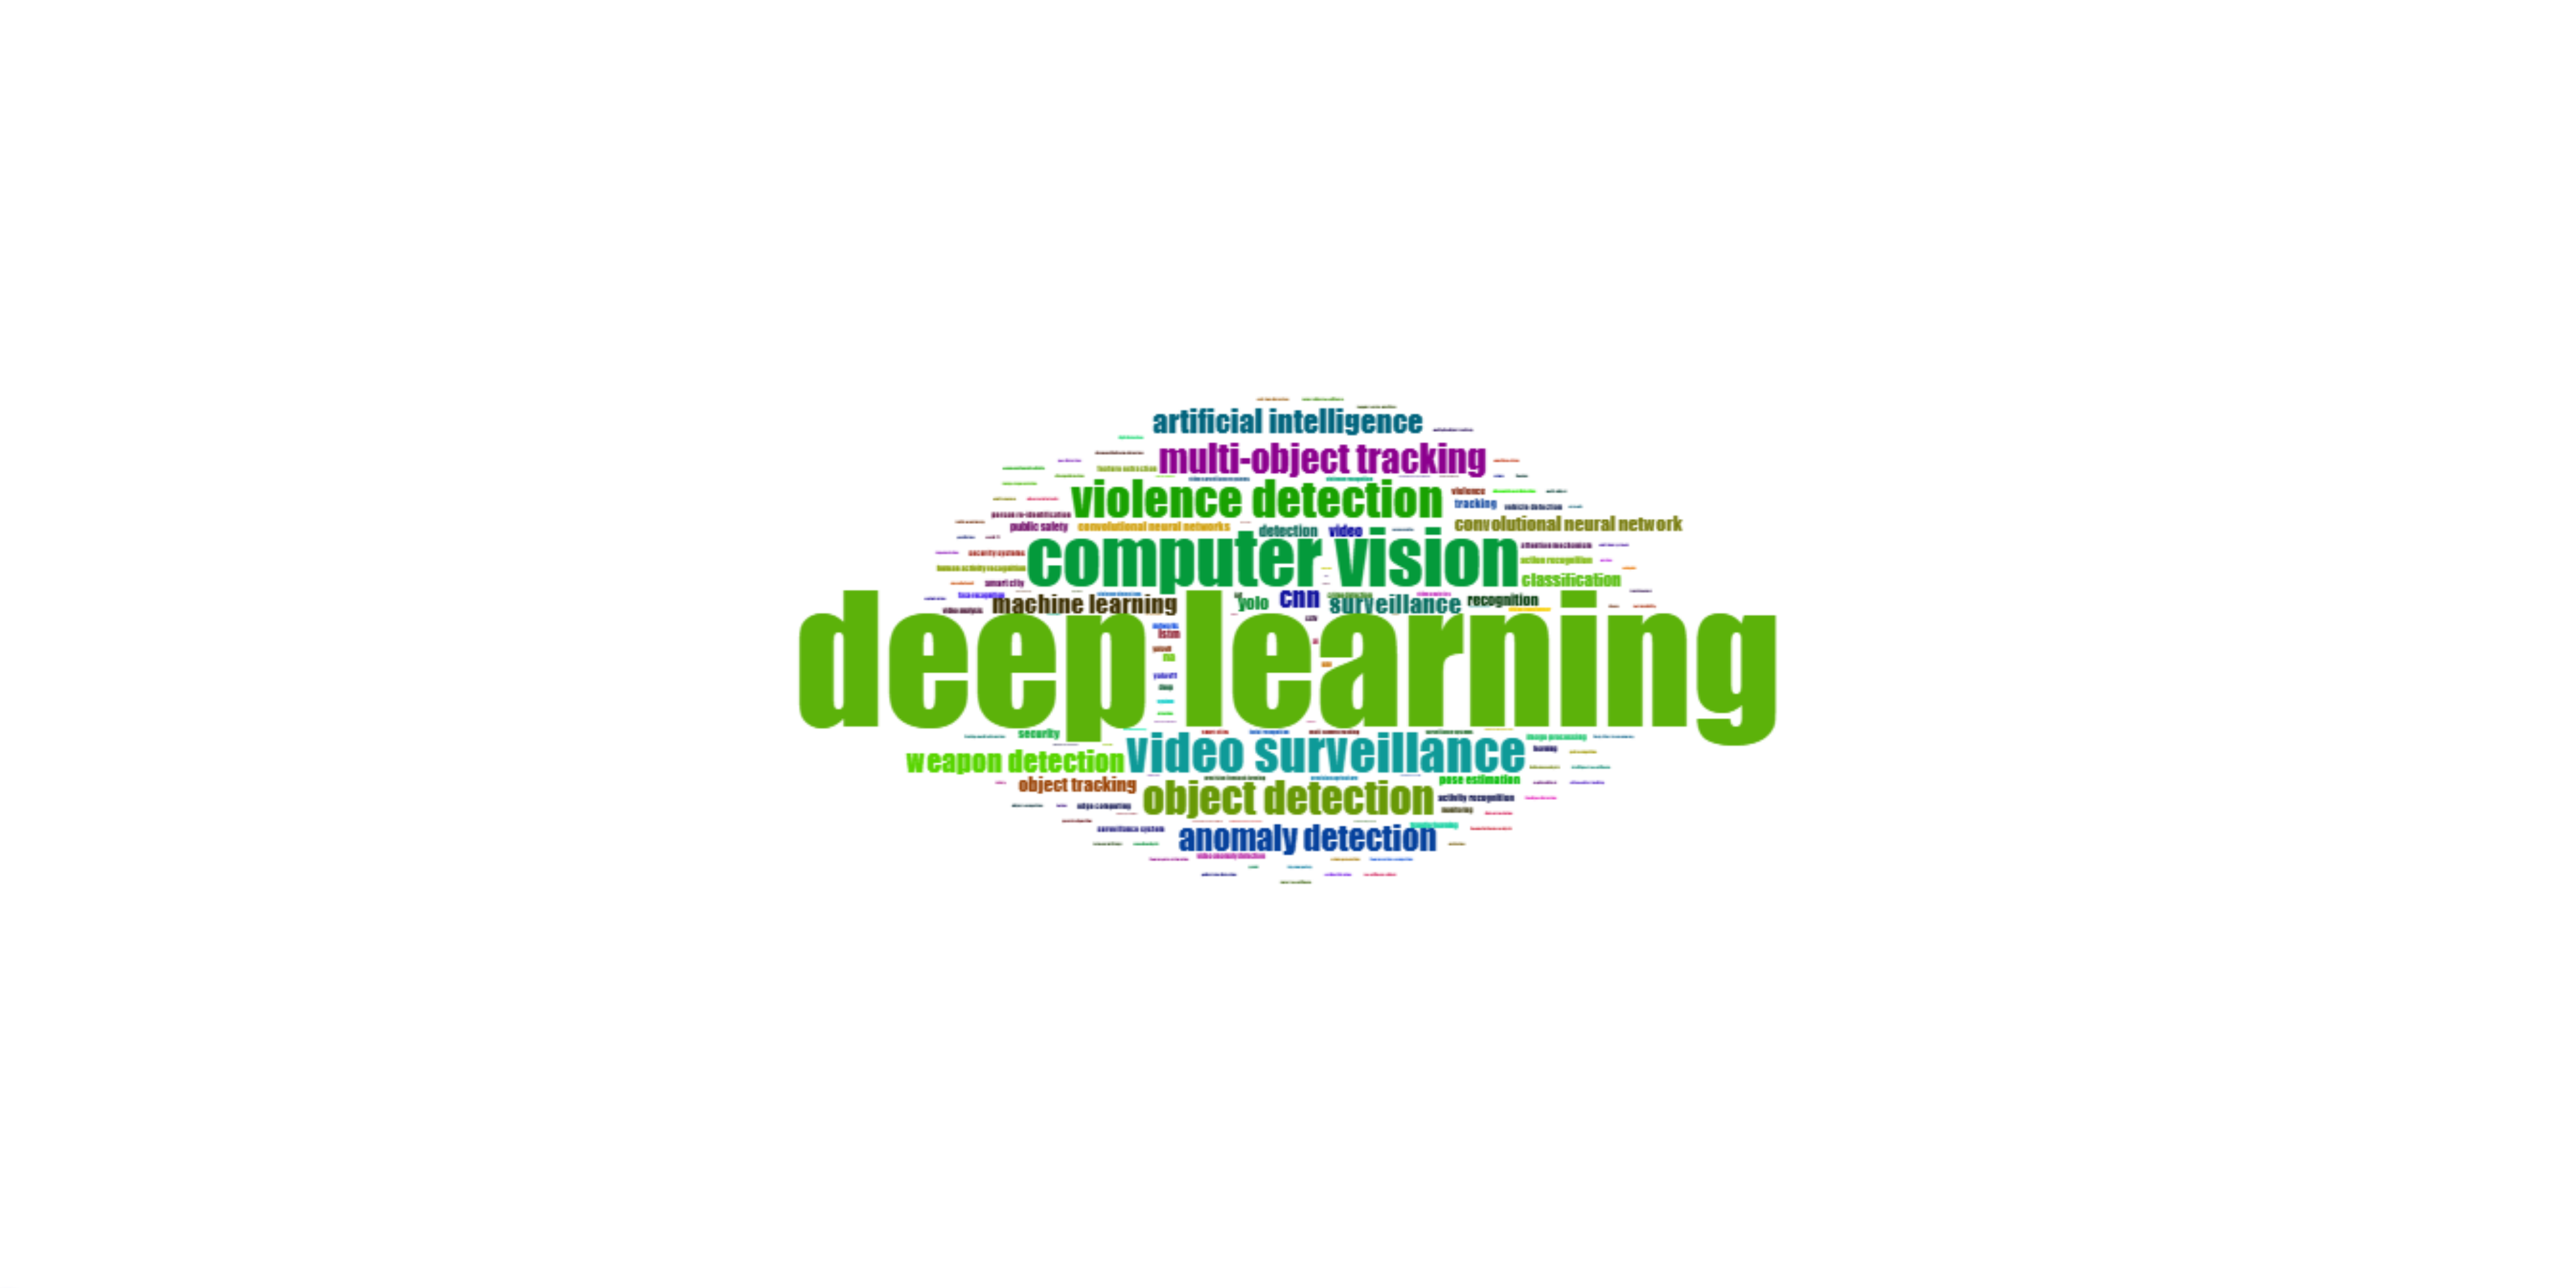
\includegraphics[width=0.90\linewidth]
{WordCloud-2026-10-04215400.72303.png}
\caption{Nube de palabras de los principales términos del corpus bibliométrico.}
\label{fig:wordcloud}
\end{figure}


% ============================================================
% SÍNTESIS DE RESULTADOS
% ============================================================

\subsubsection*{Síntesis de los principales resultados}
\label{subsec:results_synthesis}

La integración de los resultados de la revisión sistemática y del análisis
bibliométrico muestra que la investigación reciente sobre videovigilancia inteligente
se concentra principalmente en la detección automática de violencia, armas y
comportamientos anómalos mediante técnicas de aprendizaje profundo.

Las CNN bidimensionales, los detectores YOLO, las arquitecturas recurrentes y las
3D-CNN constituyen las familias tecnológicas más frecuentes. De manera coherente,
el análisis conceptual identifica \textit{deep learning}, \textit{video surveillance},
\textit{violence detection}, \textit{computer vision} y
\textit{weapon detection} como parte del núcleo temático de la literatura analizada.

No obstante, los resultados también evidencian una diferencia entre el desempeño
experimental reportado y el grado de madurez de las soluciones. Aunque 58 de los
99 estudios declararon o demostraron procesamiento en tiempo real, únicamente
21 describieron una arquitectura de despliegue y ninguno documentó una operación
sostenida en producción.

Asimismo, el predominio de datasets públicos y la limitada cantidad de evaluaciones
\textit{cross-dataset} indican que la generalización entre dominios continúa siendo
un aspecto poco evaluado. Las capacidades de seguimiento, identificación y,
especialmente, re-identificación presentan además una representación menor que las
tareas de detección.

En conjunto, los hallazgos muestran un campo con una producción científica creciente
y un desarrollo consolidado de modelos orientados a detección y reconocimiento de
eventos de seguridad, aunque persisten vacíos relacionados con validación en escenarios
reales, generalización entre conjuntos de datos, métricas especializadas de seguimiento
y documentación de arquitecturas completas de despliegue.

\section{Discussion}\label{sec12}

Discussions should be brief and focused. In some disciplines use of Discussion or `Conclusion' is interchangeable. It is not mandatory to use both. Some journals prefer a section `Results and Discussion' followed by a section `Conclusion'. Please refer to Journal-level guidance for any specific requirements. 

\section{Conclusion}\label{sec13}

Conclusions may be used to restate your hypothesis or research question, restate your major findings, explain the relevance and the added value of your work, highlight any limitations of your study, describe future directions for research and recommendations. 

In some disciplines use of Discussion or 'Conclusion' is interchangeable. It is not mandatory to use both. Please refer to Journal-level guidance for any specific requirements. 

\backmatter

\bmhead{Supplementary information}

If your article has accompanying supplementary file/s please state so here. 

Authors reporting data from electrophoretic gels and blots should supply the full unprocessed scans for key as part of their Supplementary information. This may be requested by the editorial team/s if it is missing.

Please refer to Journal-level guidance for any specific requirements.

\bmhead{Acknowledgements}

Acknowledgements are not compulsory. Where included they should be brief. Grant or contribution numbers may be acknowledged.

Please refer to Journal-level guidance for any specific requirements.

\section*{Declarations}

Some journals require declarations to be submitted in a standardised format. Please check the Instructions for Authors of the journal to which you are submitting to see if you need to complete this section. If yes, your manuscript must contain the following sections under the heading `Declarations':

\begin{itemize}
\item Funding
\item Conflict of interest/Competing interests (check journal-specific guidelines for which heading to use)
\item Ethics approval and consent to participate
\item Consent for publication
\item Data availability 
\item Materials availability
\item Code availability 
\item Author contribution
\end{itemize}

\noindent
If any of the sections are not relevant to your manuscript, please include the heading and write `Not applicable' for that section. 

%%===================================================%%
%% For presentation purpose, we have included        %%
%% \bigskip command. Please ignore this.             %%
%%===================================================%%
\bigskip
\begin{flushleft}%
Editorial Policies for:

\bigskip\noindent
Springer journals and proceedings: \url{https://www.springer.com/gp/editorial-policies}

\bigskip\noindent
Nature Portfolio journals: \url{https://www.nature.com/nature-research/editorial-policies}

\bigskip\noindent
\textit{Scientific Reports}: \url{https://www.nature.com/srep/journal-policies/editorial-policies}

\bigskip\noindent
BMC journals: \url{https://www.biomedcentral.com/getpublished/editorial-policies}
\end{flushleft}

\begin{appendices}

\section{Section title of first appendix}\label{secA1}

An appendix contains supplementary information that is not an essential part of the text itself but which may be helpful in providing a more comprehensive understanding of the research problem or it is information that is too cumbersome to be included in the body of the paper.

%%=============================================%%
%% For submissions to Nature Portfolio Journals %%
%% please use the heading ``Extended Data''.   %%
%%=============================================%%

%%=============================================================%%
%% Sample for another appendix section			       %%
%%=============================================================%%

%% \section{Example of another appendix section}\label{secA2}%
%% Appendices may be used for helpful, supporting or essential material that would otherwise 
%% clutter, break up or be distracting to the text. Appendices can consist of sections, figures, 
%% tables and equations etc.

\end{appendices}

%%===========================================================================================%%
%% If you are submitting to one of the Nature Portfolio journals, using the eJP submission   %%
%% system, please include the references within the manuscript file itself. You may do this  %%
%% by copying the reference list from your .bbl file, paste it into the main manuscript .tex %%
%% file, and delete the associated \verb+\bibliography+ commands.                            %%
%%===========================================================================================%%

\bibliography{snbibliography,methodology10_refs,core35_refs}% common bib file
%% if required, the content of .bbl file can be included here once bbl is generated
%%\input sn-article.bbl

\end{document}
